\documentclass[11pt,oneside]{book}
\let\cleardoublepage\clearpage
%\usepackage[a4paper, margin=1.2in]{geometry}
\usepackage[a4paper,top=1.9cm, bottom=1.9cm, right=1.9cm, left=1.9cm]{geometry}

\setcounter{secnumdepth}{1}

\usepackage{amsmath,amssymb}
\usepackage[amsmath]{ntheorem}
\usepackage{fontspec}
\usepackage{unicode-math}
\setmainfont{TeX Gyre Pagella}
\setmathfont{TeX Gyre Pagella Math}
\usepackage[dvipsnames]{xcolor}
\usepackage{listings}
\usepackage{courier}
\usepackage[hyphens]{url}
\usepackage{textcomp}
\usepackage{upquote}
\usepackage{graphicx}
\usepackage{tikz}
\usepackage{anyfontsize}
\usepackage{tcolorbox}
\usepackage{setspace}
\usepackage[skip=10pt plus1pt, indent=0pt]{parskip}
\usepackage{booktabs}
\usepackage{mathtools}
\usepackage{annotate-equations}
\usepackage{subcaption}
\usepackage[leftcaption]{sidecap}
\usepackage{soul}
\usepackage{relsize}
\usepackage{wrapfig}
\usepackage{marginnote}
\usepackage{titlesec}
\usepackage{tabularx}
\usepackage{multirow}
\usepackage{rotating}
\usepackage{fancyhdr}
\usepackage{float}
\usepackage{enumitem}
\usepackage[colorlinks=true,linkcolor=black,anchorcolor=black,citecolor=black,filecolor=black,menucolor=black,runcolor=black,urlcolor=black,backref=page]{hyperref}
\usepackage{emoji}
% \setemojifont{Noto Color Emoji}

\usepackage{siunitx}

\sisetup{
    group-separator={\,},
    group-minimum-digits=4,
    table-number-alignment=center,
    table-format=6.4
}

% Titlesec configuration
\titlespacing\section{0pt}{10pt plus 4pt minus 2pt}{10pt plus 4pt minus 2pt}
\titlespacing\subsection{0pt}{8pt plus 3pt minus 1pt}{8pt plus 3pt minus 1pt}

% Paragraph and spacing configuration
% \setstretch{1.25}
% \setlength{\parskip}{0pt}
% \setlength{\parindent}{0pt} % Disable indentation globally

% Widows and orphans control
% \clubpenalty=10000
% \widowpenalty=10000
% \displaywidowpenalty=10000

% \tcbset {
% base/.style={
%     arc=0mm, 
%     bottomtitle=0.5mm,
%     boxrule=0mm,
%     colbacktitle=black!10!white, 
%     coltitle=black, 
%     fonttitle=\bfseries, 
%     left=2.5mm,
%     leftrule=1mm,
%     right=3.5mm,
%     title={#1},
%     toptitle=0.75mm, 
% }
% }
% colors
\definecolor{drawgray}{HTML}{666666}
\definecolor{drawgray_l}{HTML}{F5F5F5}
\definecolor{drawblue}{HTML}{6C8EBF}
\definecolor{drawblue_l}{HTML}{DAE8FC}
\definecolor{drawgreen}{HTML}{82B366}
\definecolor{drawgreen_l}{HTML}{D5E8D4}
\definecolor{draworange}{HTML}{D79B00}
\definecolor{draworange_l}{HTML}{FFE6CC}
\definecolor{drawyellow}{HTML}{D6B656}
\definecolor{drawyellow_l}{HTML}{FFF2CC}
\definecolor{drawred}{HTML}{B85450}
\definecolor{drawred_l}{HTML}{EA6B66}
\definecolor{drawviolet}{HTML}{9673A6}
\definecolor{drawviolet_l}{HTML}{E1D5E7}
\definecolor{drawblackish}{HTML}{422222}

\definecolor{deepblue}{rgb}{0,0,0.5}
\definecolor{deepgreen}{rgb}{0,0.5,0}

\tcbset {
  base/.style={
    arc=0mm, 
    bottomtitle=0.5mm,
    boxrule=0mm,
    colbacktitle=drawblue_l, 
    colframe=drawblue,
    coltitle=black,
    fonttitle=\bfseries, 
    left=2.5mm,
    leftrule=1mm,
    right=3.5mm,
    title={#1},
    toptitle=0.75mm, 
  }
}

\newtcolorbox{supportbox}[1]{
  colframe=drawblue, 
  base={#1}
}

\definecolor{brandblue}{rgb}{0.34, 0.7, 1}
\newtcolorbox{mainbox}[1]{
colframe=brandblue, 
base={#1}
}

\newtcolorbox{subbox}[1]{
colframe=black!30!white,
base={#1}
}

\usepackage[style=0,ntheorem]{mdframed}
\mdfsetup{%
topline=false,
rightline=false,
bottomline=false,
linewidth=3pt,
innerleftmargin=15pt,
innerrightmargin=0pt,
skipabove=\baselineskip,
skipabove=1.2\baselineskip,
}
\newmdtheoremenv[linecolor=drawred]{definition}{Definition}[chapter]

\hypersetup{
    colorlinks=true,
    linkcolor=drawblackish,
    breaklinks=true,
    citecolor = drawblackish,
    urlcolor=drawblue,
}

% 1.10 spacing
\setstretch{1.10}

% Fancy header
\usepackage{fancyhdr}
\renewcommand{\chaptermark}[1]{\markboth{#1}{}}
\renewcommand{\sectionmark}[1]{\markright{#1}}
\fancyhead{} % clear all header fields
\fancyhead[LE]{{\color{black!40}\thepage}}
\fancyhead[RE]{\bfseries\normalfont {\color{black!40}\nouppercase{\rightmark}}}
\fancyhead[LO]{\bfseries\normalfont {\color{black!40}\nouppercase{Chapter \thechapter: \leftmark}}}
\fancyhead[RO]{{\color{black!40}\thepage}}

% Chapter title
\usepackage{titlesec, blindtext, color}
\definecolor{gray75}{gray}{0.75}
\newcommand{\hsp}{\hspace{20pt}}
% \titleformat{\chapter}[hang]{\Huge\bfseries}{\selectfont \thechapter\hsp\textcolor{red}{\emoji{open-book}}\hsp}{0pt}{\Huge\bfseries}

\begin{document}

% \captionsetup[figure]{margin=1.5cm,font=small,labelfont={bf},name={Figure},labelsep=colon,textfont={it}}
% \captionsetup[table]{margin=1.5cm,font=small,labelfont={bf},name={Table},labelsep=colon,textfont={it}}

% diminuire il margine superiore della pagina mantenendo il margine inferiore
\newgeometry{top=2cm, bottom=2cm, right=2cm, left=2cm}

\begin{titlepage}
	\begin{center}
		
\includegraphics[width=0.6\textwidth]{figures/uniba_logo.png}\\
		\vspace{1cm}
		% Dipartimento
		{\large Computer Science Department}\\
		\vspace{1cm}
		% Corso di laurea
		{\large Master Degree in Computer Science}\\
		\vspace{1cm}
		\hrule
		\vspace{1.5cm}
		%{\large \textbf{LECTURE NOTES ON}}\\
		\vspace{0.5cm}
		% Materia
		{\large PROJECT DOCUMENTATION for \underline{BIG DATA}}\\
		\vspace{1.5cm}
		% Titolo
		{\LARGE \textbf{Evaluating Temporal Link Prediction methods to generate synthetic social networks data}}\\
		{\large \textit{}}\\
		\vspace{1.2cm}

		\vfill

		\begin{tabularx}{\textwidth}{@{}Xr@{}}
			% Laureando e Relatori
			{\large Author:}               \\
			\vspace{0.1cm}
			{\large \textbf{Mattia Curri}} \\ \\
		\end{tabularx}

		\vspace{0.8cm}
		\hrule
		\vspace{0.8cm}
		% Anno accademico in cui si è iscritti
		{\large ACADEMIC YEAR \textbf{2025{-}2026}}
	\end{center}
\end{titlepage}
\restoregeometry
\pagestyle{empty}
{
	\tableofcontents
}
%\newpage
\mainmatter

\titleformat{\chapter}[hang]{\Huge\bfseries}{\selectfont \thechapter\hsp\textcolor{red}{\emoji{moneybag}}\hsp}{0pt}{\Huge\bfseries}

\chapter{Business Understanding}

This chapter covers the business understanding phase of the CRISP-DM methodology.

\section{Determine Business Objectives}

\subsection*{Background}
Social network analysis (SNA) has emerged as a critical pursuit in understanding the complex dynamics of modern online communities. While traditional statistical techniques remain valuable, SNA introduces specialized measures to capture the dependencies between social entities, characterize their behaviors, and assess their impact on the network both structurally and temporally~\cite{tabassumSocialNetworkAnalysis2018}. The fundamental principle of SNA lies in shifting the analytical focus from individual social actors to the relationships and interactions that bind them, revealing patterns that emerge from the network's underlying structure rather than from isolated entities~\cite{tabassumSocialNetworkAnalysis2018}.

In the globalized digital landscape, social networks have become one of the favorite means for modern society to perform social interactions and exchange information via the Internet, allowing people to share their contents without boundaries~\cite{daudApplicationsLinkPrediction2020,pellicaniSAIRUSSpatiallyawareIdentification2023}. Through these platforms, individuals communicate and express their comments, likes, and interests in a fast and easy manner, creating complex connections that can be immediately visualized as large graphs~\cite{daudApplicationsLinkPrediction2020}. This massive spread of social media has introduced unprecedented opportunities for information dissemination~\cite{khanGraphNeuralNetworks2024}. However, this very interconnectedness presents significant challenges: the same platforms that facilitate legitimate social connections also provide powerful tools for malicious activities, including misinformation campaigns, cyberbullying, hate speech propagation, and the radicalization of vulnerable individuals~\cite{benedettiMultiviewLearningIdentification2025,pellicaniSAIRUSSpatiallyawareIdentification2023,khanGraphNeuralNetworks2024,benedettiIMMENSEInductiveMultiperspective2025}.

Risky users exploit the spreading power of social networks for illegal or harmful activities such as inciting religious or political extremism, disseminating disinformation, or recruiting. For these reasons, detecting them has become a fundamental task for ensuring the safe use of these platforms~\cite{pellicaniSAIRUSSpatiallyawareIdentification2023,benedettiMultiviewLearningIdentification2025,benedettiIMMENSEInductiveMultiperspective2025}. This challenge is particularly acute when dealing with borderline users who appear risky from certain perspectives but not from others, and is further complicated by the dynamic nature of social networks~\cite{pellicaniSAIRUSSpatiallyawareIdentification2023,benedettiMultiviewLearningIdentification2025}. User relationships, content semantics, and behavioral patterns continuously evolve; models that treat networks as static entities fail to capture users who transition from safe to radicalized behavior over time~\cite{benedettiMultiviewLearningIdentification2025}.

The unstructured nature of user interactions on social media platforms renders manual identification of malicious actors both tedious and impractical at scale~\cite{khanGraphNeuralNetworks2024}. Recent research has increasingly focused on leveraging graph-based representations, where users constitute nodes and their interactions form edges, to address this complexity~\cite{khanGraphNeuralNetworks2024,corizzoHURIHybridUser2023}. Link prediction, defined as the process of predicting future connections between pairs of unconnected links based on existing connections~\cite{daudApplicationsLinkPrediction2020}, represents a fundamental problem in network analysis that has evolved from static snapshot-based approaches to temporal methodologies that exploit multiple network states across time to predict future or re-occurring connections~\cite{tabassumSocialNetworkAnalysis2018,daudApplicationsLinkPrediction2020}. This temporal perspective aligns with the recognition that real-world networks are not static but dynamic and continuously evolving, requiring analytical frameworks that can capture growth patterns and temporal dependencies~\cite{tabassumSocialNetworkAnalysis2018}.

Given the urgency of protecting society from exposure to discriminatory, hateful, and violent content at the massive scale of contemporary social networks, there is a critical need for effective automated systems to assist Law Enforcement Agencies in identifying and addressing users who disseminate malicious content~\cite{benedettiIMMENSEInductiveMultiperspective2025}. This work addresses this need by developing methods that integrate multiple perspectives of user behavior, account for the temporal evolution of networks, and leverage the relational structure inherent in social media platforms to enable accurate and timely identification of risky users.


\subsection*{Business Goals}
The primary business goal of this project is to develop an effective temporal link prediction system for social networks that can:

\begin{itemize}
    \item Predict future connections between users based on their historical interactions and content
    \item Evaluate the effectiveness of incremental learning approaches for temporal network evolution
    \item Given a dataset of users and relative posts, generate realistic synthetic social network structures
    \item Provide insights into how network properties evolve over time
\end{itemize}

\subsection*{Business Success Criteria}
The project will be considered successful if it achieves the following outcomes:

\begin{itemize}
    \item Development of a temporal link prediction model based on EvolveGCN
    \item Quantitative comparison of model performance using standard metrics (Mean Average Precision, AUC, Precision, Recall, F1)
    \item Successful transfer learning application: trained models can generate plausible network structures on synthetic datasets
    \item Analysis of network evolution patterns and structural properties across temporal snapshots
    \item Generation of a large synthetic network of 1000 artificial users with realistic connection patterns
\end{itemize}

\section{Assess Situation}

\subsection*{Inventory of Resources}

The available data are being collected from the social network platform Gab\footnote{\url{https://gab.com/}}, known for its minimal content moderation policies and popularity among far-right communities. The dataset includes user profiles, posts, and interaction data (likes, comments, shares) over a defined time period.

Current resources available for the project are the following machines:

\begin{enumerate}
    \item CPU: AMD Ryzen 7 7700, 8 cores, 16 threads; GPU: NVIDIA RTX 5060Ti, 16 GB VRAM; RAM: 48 GB
    \item CPU: AMD Ryzen 7 7840HS, 8 cores, 16 threads; GPU: Integrated AMD Radeon 780M; RAM: 48 GB
    \item CPU: Intel Core i7-10750H, 6 cores, 12 threads; GPU: NVIDIA GTX 1650 Mobile Max-Q, 4 GB VRAM; RAM: 16 GB
\end{enumerate}

\subsection*{Identify Constraints}

There are no significant constraints anticipated for this project. However, potential challenges include:

\begin{itemize}
    \item Data Quality: The collected data may contain noise, missing values, or inconsistencies that could affect model performance.
    \item Computational Resources: Training complex models on large datasets may require significant computational power and time.
    \item Ethical Considerations: Handling user data requires adherence to privacy regulations and ethical guidelines to ensure responsible use of information.
\end{itemize}

\subsection*{Assumptions}

\begin{itemize}
    \item The dataset from Gab is representative of broader social network dynamics and user behaviors.
    \item A connection between users exists if they are connected in one snapshot
    \item Graphs are undirected and unweighted
    \item If a connection exists between two users in a snapshot, it will also exist in all subsequent snapshots
\end{itemize}


\section{Determine Data Mining Goals}

\subsection*{Data Mining Goals}

Here we translate the business goals into specific data mining objectives:

\begin{itemize}
    \item Develop a temporal link prediction model using EvolveGCN to forecast future user connections based on historical interaction data.
    \item Evaluate the model's performance using metrics such as Mean Average Precision (MAP), Area Under the Curve (AUC), Precision, Recall, and F1-score.
    \item Adapt and test the trained model for generating synthetic social network structures.
    \item Analyze the temporal evolution of network properties, including degree distribution, clustering coefficient, and average path length.
\end{itemize}

\subsection*{Success Criteria}

The success of the data mining efforts will be measured by:

\begin{itemize}
    \item Achieving high performance on link prediction tasks
    \item Demonstrating the model's ability to generalize to synthetic datasets, producing realistic network structures.
    \item Providing comprehensive insights into the temporal dynamics of the social network through detailed analysis of evolving network metrics.
\end{itemize}
\titleformat{\chapter}[hang]{\Huge\bfseries}{\selectfont \thechapter\hsp\textcolor{red}{\emoji{open-book}}\hsp}{0pt}{\Huge\bfseries}

\chapter{Data Understanding}

This chapter covers the data understanding phase of the CRISP-DM methodology.

\section{Collect Initial Data}

The available data are being collected from the social network platform Gab\footnote{\url{https://gab.com/}}. The dataset includes several snapshots, in particular, \texttt{2016-2021}, \texttt{2022}, \texttt{2023}, \texttt{2024}, \texttt{January-July 2025} and \texttt{July 2025}. For every snapshot, there three files:

\begin{itemize}
	\item \texttt{posts\_current\_snapshot.csv}: contains all the posts made by users in the platform for that snapshot;
	\item \texttt{posts\_incremental.csv}: contains all the posts made by users in the platform since the previous snapshots up to the current one;
	\item \texttt{social\_network.edg}: contains the social network graph in edge list format, where every line represents a directed edge from a follower to a followee (X follows Y).
\end{itemize}

Along with them, there are also 3 synthetic batches for the subsequent task of using the trained model on the original data to generate links.

\section{Describe Data}

Raw data files are in CSV format, with the exception of the social network graph which is in edge list format. For each post, the following attributes are available:

\begin{itemize}
	% \item \texttt{unnamed\_0} (autoincrement): index of the post, autoincremented
	\item \texttt{id} (integer): unique identifier of the post
	\item \texttt{content} (string): text of the post
	\item \texttt{account\_id} (integer): unique identifier of the user who made the post
	\item \texttt{created\_at} (string): ISO 8601 timestamp of when the post was created
	\item \texttt{language} (string): language code of the post
	\item \texttt{replies\_count} (integer): number of replies to the post
	\item \texttt{reblogs\_count} (integer): number of reblogs of the post
	\item \texttt{reactions\_counts} (string): JSON dictionary of reactions to the post
	\item \texttt{quotes\_count} (integer): number of quotes of the post
	\item \texttt{timestamp} (string): ISO 8601 timestamp of the post (\texttt{created\_at} + timezone)
\end{itemize}


\section{Explore Data}

% The exploration of the dataset involves analyzing temporal patterns, content characteristics, user engagement, and activity distributions across all snapshots.

\sethlcolor{cyan!60}
The dataset had been preprocessed before: posts lacking textual content, posts containing images or videos, and posts written in languages other than English were removed. HTML tags were also stripped from the remaining content.


\subsection*{Temporal Distribution}

The dataset spans from August 22, 2016 to August 2, 2025, covering a period of approximately 9 years. Table~\ref{tab:temporaldistribution} summarizes the temporal distribution across all snapshots.

\begin{table}[H]
	\centering
	\caption{Temporal distribution of posts across snapshots}
	\label{tab:temporaldistribution}
	\begin{tabular}{lrrr}
		\toprule
		\textbf{Snapshot} & \textbf{Posts} & \textbf{Time Span (days)} & \textbf{Max Gap (days)} \\
		\midrule
		2016-2021         & 18,926         & 1,957                     & 49                      \\
		2022              & 13,108         & 364                       & $<$1                    \\
		2023              & 13,376         & 364                       & $<$1                    \\
		2024              & 13,400         & 365                       & $<$1                    \\
		Jan-Jul 25        & 44,878         & 180                       & $<$1                    \\
		Jul 25            & 78,857         & 32                        & $<$1                    \\
		\bottomrule
	\end{tabular}
\end{table}

The early snapshot (2016-2021) shows significant temporal gaps, with 39 gaps of 7 or more days detected, reflecting the sparse data collection in the platform's early years. From 2022 onwards, the data collection became more consistent, with no gaps exceeding one day. The volume of posts shows a marked increase over time, with the Jul 25 snapshot alone containing more posts than all previous years combined.

\subsection*{Completeness Analysis}

\subsubsection{Missing Values}

The dataset shows excellent completeness for most attributes. The only attribute with missing values is \texttt{language}, with 877 missing values (0.48\%) in the aggregated current snapshots and 3,747 (0.85\%) in the incremental data. All other attributes are 100\% complete.

\begin{table}[H]
	\centering
	\caption{Missing values summary (aggregated current snapshots)}
	\label{tab:missing_values}
	\begin{tabular}{lrr}
		\toprule
		\textbf{Attribute}   & \textbf{Missing Count} & \textbf{Missing \%} \\
		\midrule
		language             & 877                    & 0.48\%              \\
		All other attributes & 0                      & 0.00\%              \\
		\bottomrule
	\end{tabular}
\end{table}

The missing \texttt{language} values likely correspond to posts where automatic language detection failed, possibly due to very short content, mixed-language posts, or non-standard text.

\subsubsection{No Empty Content}

Importantly, no posts with empty \texttt{content} fields were found, ensuring all records contain textual data for analysis.

\subsection*{Consistency Checks}

\subsubsection{Snapshot vs. Incremental Consistency}

A critical quality check verified that each current snapshot is fully contained within its corresponding incremental file. As shown in Table~\ref{tab:consistency}, all six snapshots achieved 100\% coverage:

\begin{table}[H]
	\centering
	\caption{Consistency verification}
	\label{tab:consistency}
	\begin{tabular}{lrrr}
		\toprule
		\textbf{Snapshot} & \textbf{Snapshot Posts} & \textbf{Incremental Posts} & \textbf{Coverage} \\
		\midrule
		2016-2021         & 18,926                  & 18,926                     & 100\%             \\
		2022              & 13,108                  & 32,034                     & 100\%             \\
		2023              & 13,376                  & 45,410                     & 100\%             \\
		2024              & 13,400                  & 58,810                     & 100\%             \\
		Jan-Jul 25        & 44,878                  & 103,688                    & 100\%             \\
		Jul 25            & 78,857                  & 182,545                    & 100\%             \\
		\bottomrule
	\end{tabular}
\end{table}

\subsubsection{Temporal Consistency}

The \texttt{created\_at} and \texttt{timestamp} fields are identical across all snapshots, confirming consistent timestamp handling. No posts with future dates were detected.

\subsubsection{Unique Identifiers}

No duplicate post IDs were found, either within individual snapshots or across the aggregated dataset. Each post maintains a unique identifier throughout the dataset.

\subsection*{Duplicate Content Analysis}

While post IDs are unique, content-level duplicates exist in the dataset. Table~\ref{tab:duplicates} summarizes the duplicate content findings.

\begin{table}[H]
	\centering
	\caption{Duplicate content analysis per snapshot}
	\label{tab:duplicates}
	\begin{tabular}{lrr}
		\toprule
		\textbf{Snapshot} & \textbf{Duplicate Posts} & \textbf{Percentage} \\
		\midrule
		2016-2021         & 339                      & 1.79\%              \\
		2022              & 396                      & 3.02\%              \\
		2023              & 563                      & 4.21\%              \\
		2024              & 563                      & 4.20\%              \\
		Jan-Jul 25        & 3,377                    & 7.52\%              \\
		Jul 25            & 7,919                    & 10.04\%             \\
		\bottomrule
	\end{tabular}
\end{table}

Gab treats reblogs as standalone posts. When a user reblogs a post, Gab records it as a new post with content identical to the original. The same behavior occurs on Twitter with retweets.

% The increasing duplicate rate over time suggests growing repetitive posting behavior, possibly including:
% \begin{itemize}
% 	\item Users reposting the same content multiple times;
% 	\item Common phrases or memes shared by different users;
% 	\item Automated or bot-like posting patterns.
% \end{itemize}

Importantly, no completely duplicate rows (excluding ID) were found, meaning each post has unique metadata even when content is identical.

% \subsection*{Data Type Verification}

% All attributes maintain consistent data types across snapshots:
% \begin{itemize}
% 	\item Numeric fields (\texttt{id}, \texttt{account\_id}, \texttt{replies\_count}, \texttt{reblogs\_count}, \texttt{quotes\_count}): \texttt{int64}
% 	\item Text fields (\texttt{content}, \texttt{language}, \texttt{created\_at}, \texttt{timestamp}, \texttt{reactions\_counts}): \texttt{str}
% \end{itemize}

% \subsection*{Encoding Issues}

% No encoding issues were detected in the text content. The dataset appears to be properly UTF-8 encoded, with no problematic character sequences found during quality checks.

% \subsection*{Outlier Detection}

% Several extreme values were identified but are considered legitimate data points:
% \begin{itemize}
% 	\item Maximum replies: 22,211 (highly viral post)
% 	\item Maximum reblogs: 24,464 (highly viral post)
% 	\item Maximum reactions: 116,141 (exceptionally popular content)
% 	\item Maximum text length: 11,753 characters (long-form content)
% \end{itemize}

% These outliers represent the heavy-tailed distribution typical of social media engagement, where a small number of viral posts receive disproportionate attention.

% \subsection*{Summary of Data Quality}

% The dataset demonstrates high overall quality:
% \begin{itemize}
% 	\item \textbf{Completeness}: 99.52\% complete (only \texttt{language} has missing values)
% 	\item \textbf{Consistency}: 100\% snapshot-incremental consistency; unique IDs throughout
% 	\item \textbf{Accuracy}: No encoding issues; timestamps properly formatted
% 	\item \textbf{Timeliness}: Data spans 2016-2025 with recent snapshots being most comprehensive
% \end{itemize}

% Areas requiring attention during data preparation include:
% \begin{enumerate}
% 	\item Handling the 0.48\% missing \texttt{language} values (imputation or filtering)
% 	\item Addressing content duplicates based on analysis objectives
% 	\item Considering the heavy-tailed engagement distributions for modeling purposes
% \end{enumerate}

\subsection*{Embedding Analysis}

Along with the textual data, BERT embeddings have been provided for all posts in both the real and synthetic datasets. This section analyzes the quality and distribution of these embeddings to understand their suitability for the link prediction task.

Table~\ref{tab:embedding_stats} summarizes the key statistics about the BERT embeddings for real and synthetic posts. The BERT embeddings for posts exhibit significantly different distributions between real and synthetic data.

\begin{table}[H]
	\centering
	\caption{BERT embedding statistics: Real vs Synthetic posts}
	\label{tab:embedding_stats}
	\begin{tabular}{lrr}
		\toprule
		\textbf{Metric}                        & \textbf{Real}             & \textbf{Synthetic} \\
		\midrule
		Number of posts                        & 182,545                   & 9,990              \\
		Within-group cosine similarity (mean)  & 0.821                     & 0.924              \\
		Within-group cosine similarity (std)   & 0.097                     & 0.019              \\
		Euclidean distance within-group (mean) & 6.05                      & 3.88               \\
		Within-group variance (mean per dim)   & 0.026                     & 0.010              \\
		Cross-group cosine similarity (mean)   & \multicolumn{2}{c}{0.839}                      \\
		Cross-group centroid distance          & \multicolumn{2}{c}{2.61}                       \\
		\bottomrule
	\end{tabular}
\end{table}

The most striking difference is in the within-group cosine similarity: synthetic posts show a mean similarity of 0.924 with very low standard deviation (0.019), indicating that synthetic posts are extremely homogeneous. In contrast, real posts have a mean similarity of 0.821 with much higher variance (std=0.097).

\begin{figure}[H]
	\centering
	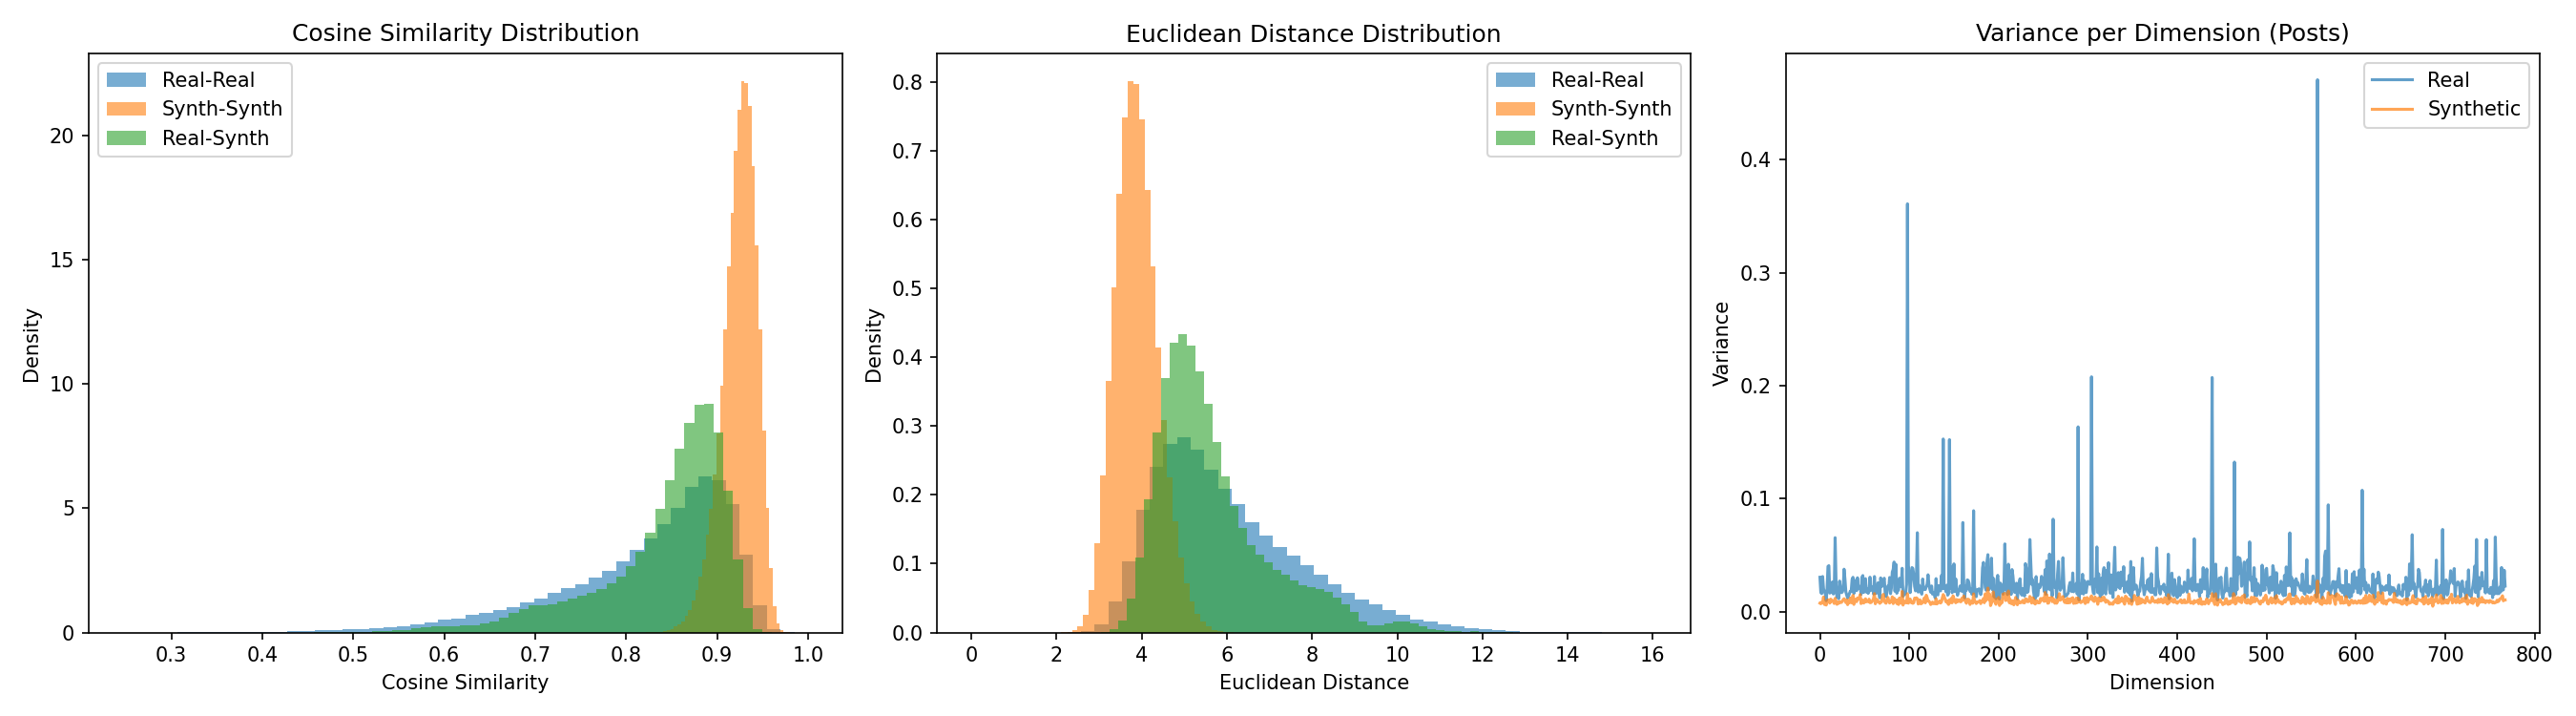
\includegraphics[width=0.9\textwidth]{figures/embedding_comparison.png}
	\caption{Comparison of cosine similarity distributions between real and synthetic embeddings. Synthetic posts cluster tightly with similarities concentrated around 0.90-0.95, while real posts show a broader distribution.}
	\label{fig:embedding_comparison}
\end{figure}

To visualize the embedding space structure, PCA and t-SNE projections were computed for both post and user-level embeddings. Figure~\ref{fig:embedding_visualization_posts} shows the post-level visualization.

\begin{figure}[H]
	\centering
	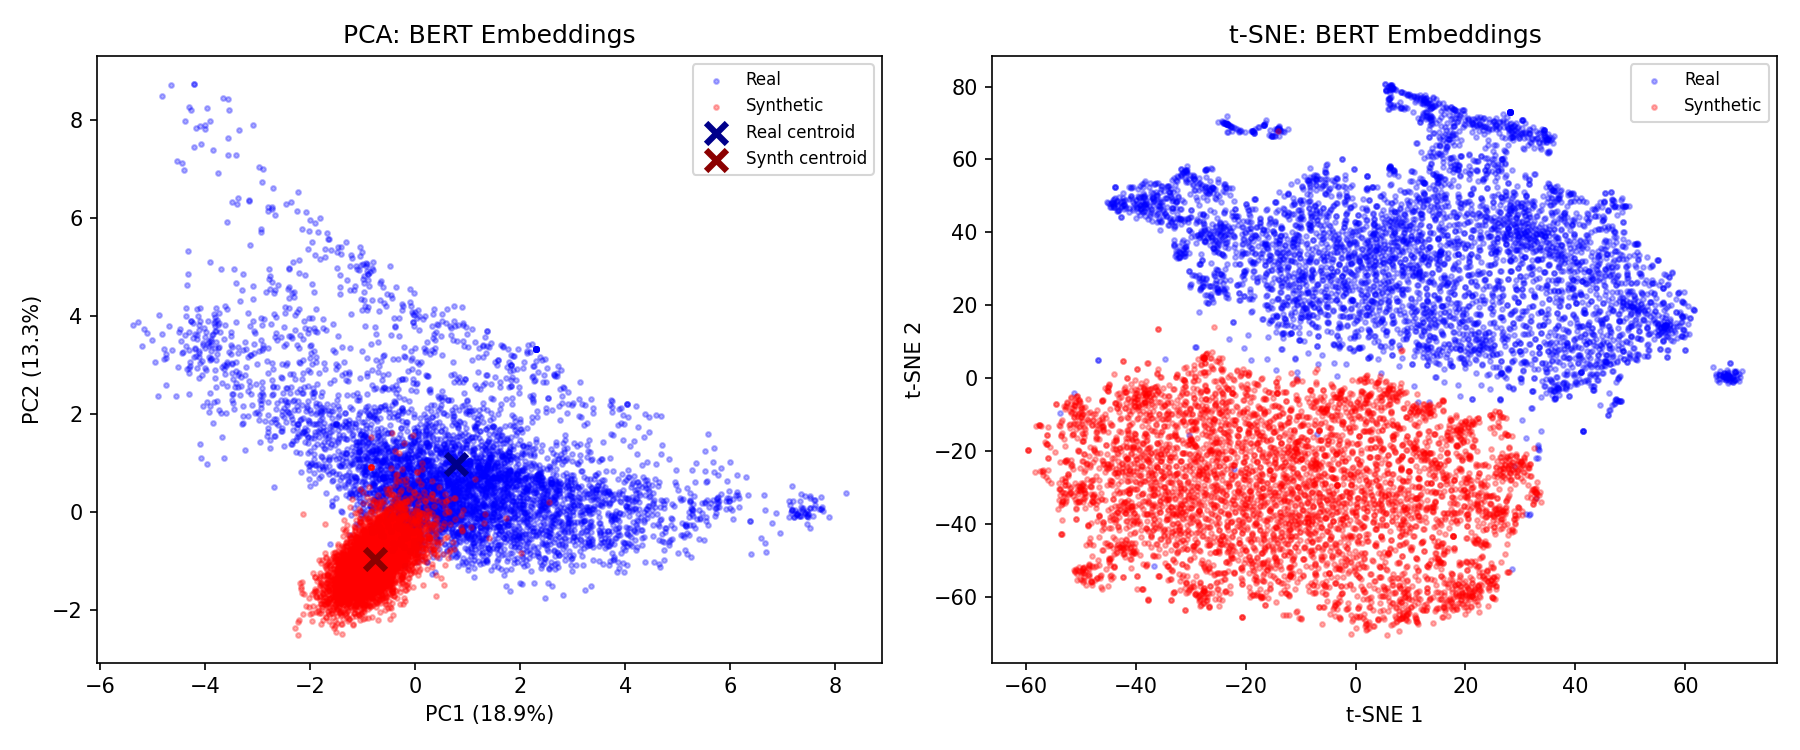
\includegraphics[width=0.95\textwidth]{figures/embeddings_visualization_bert.png}
	\caption{PCA and t-SNE visualization of post embeddings. The synthetic posts (red) form a tight, well-defined cluster, while real posts (blue) spread across a much larger region of the embedding space.}
	\label{fig:embedding_visualization_posts}
\end{figure}

Figure~\ref{fig:embedding_visualization_users} presents the user-level visualization, where the homogeneity of synthetic users becomes even more clear.

\begin{figure}[H]
	\centering
	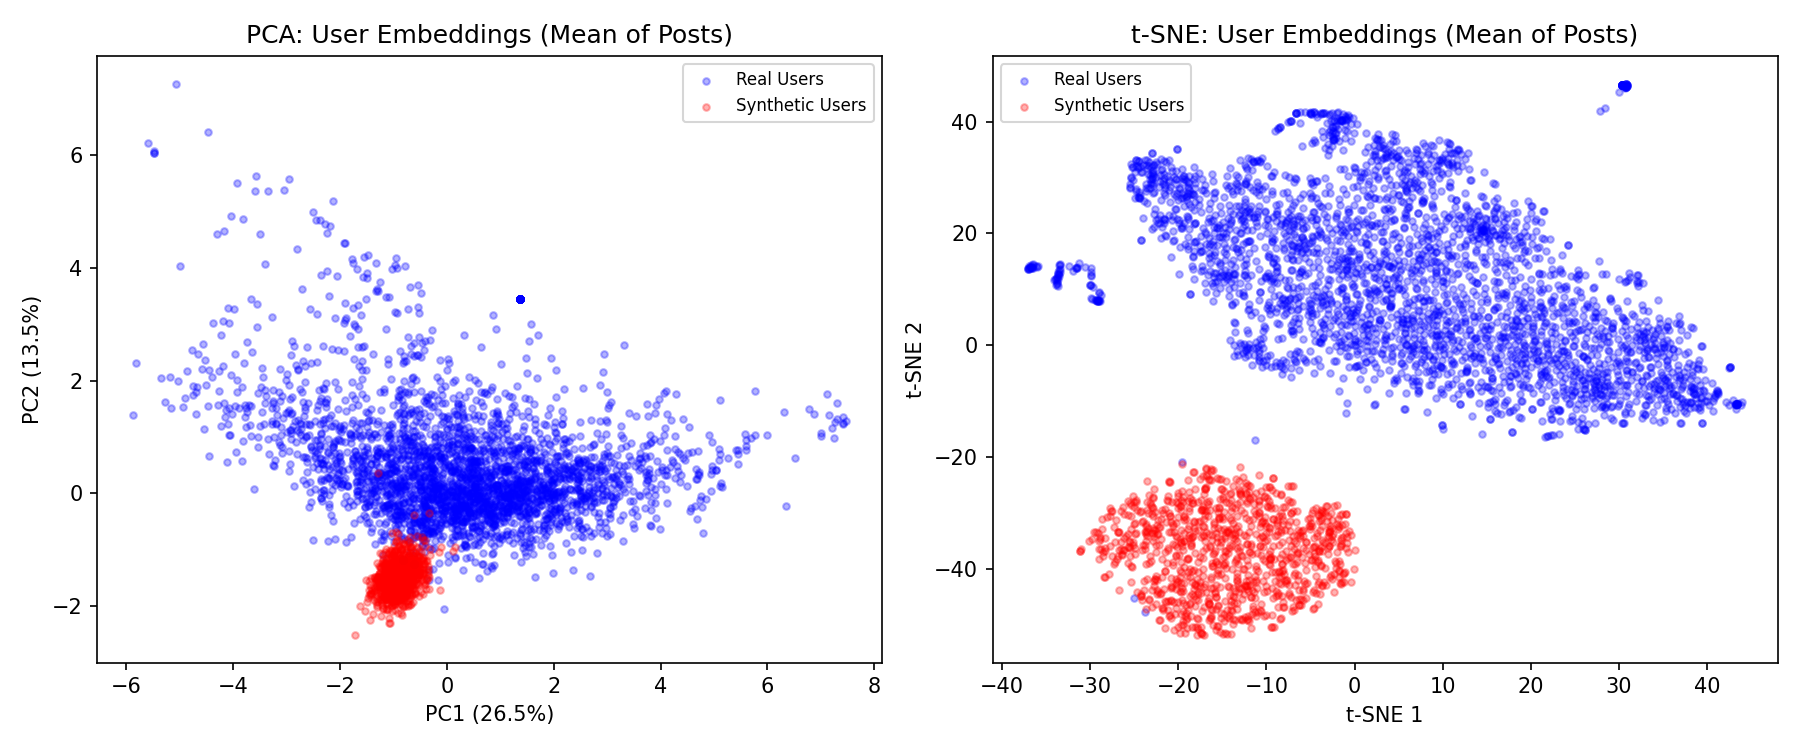
\includegraphics[width=0.95\textwidth]{figures/user_embeddings_visualization.png}
	\caption{PCA and t-SNE visualization of user embeddings (mean of posts per user). Synthetic users (red) cluster in an extremely tight region, while real users (blue) occupy a much broader space.}
	\label{fig:embedding_visualization_users}
\end{figure}

\subsection*{Variance Analysis}

Table \ref{tab:variance_comparison} provides a detailed comparison of variance metrics for both posts and users.

\begin{table}[H]
	\centering
	\caption{Variance comparison: Real vs Synthetic (posts and users)}
	\label{tab:variance_comparison}
	\begin{tabular}{lrrr}
		\toprule
		\textbf{Level}                      & \textbf{Real}            & \textbf{Synthetic} & \textbf{Ratio} \\
		\midrule
		Posts within-group variance         & 0.0264                   & 0.0099             & 2.67x          \\
		Users within-group variance         & 0.0174                   & 0.0015             & 11.23x         \\
		\midrule
		Posts cross-group centroid distance & \multicolumn{3}{c}{2.61}                                       \\
		Users cross-group centroid distance & \multicolumn{3}{c}{2.57}                                       \\
		\bottomrule
	\end{tabular}
\end{table}

The variance per embedding dimension reveals a significant difference in the representational space. For posts, the variance ratio (real/synthetic) is \textbf{2.67x}, with real posts showing a mean variance of \textbf{0.0264} per dimension compared to \textbf{0.0099} for synthetic posts.

At the user level, the disparity is even more pronounced. Table~\ref{tab:variance_comparison} presents the variance comparison for both posts and users.

We distinguish between two types of variance metrics:
\begin{itemize}
	\item \textbf{Within-group variance}: measures how much embeddings vary \textit{within} each group. For example, real user within-group variance (0.0174) indicates how much real users differ from each other. The ratio of 11.23x means synthetic users are much more homogeneous than real users.
	\item \textbf{Cross-group centroid distance}: measures the Euclidean distance between the centroids (mean embeddings) of the two groups. A distance of 2.57 for users indicates that real and synthetic users occupy distinct but not extremely distant regions of the embedding space.
\end{itemize}

% \begin{figure}[H]
% 	\centering
% 	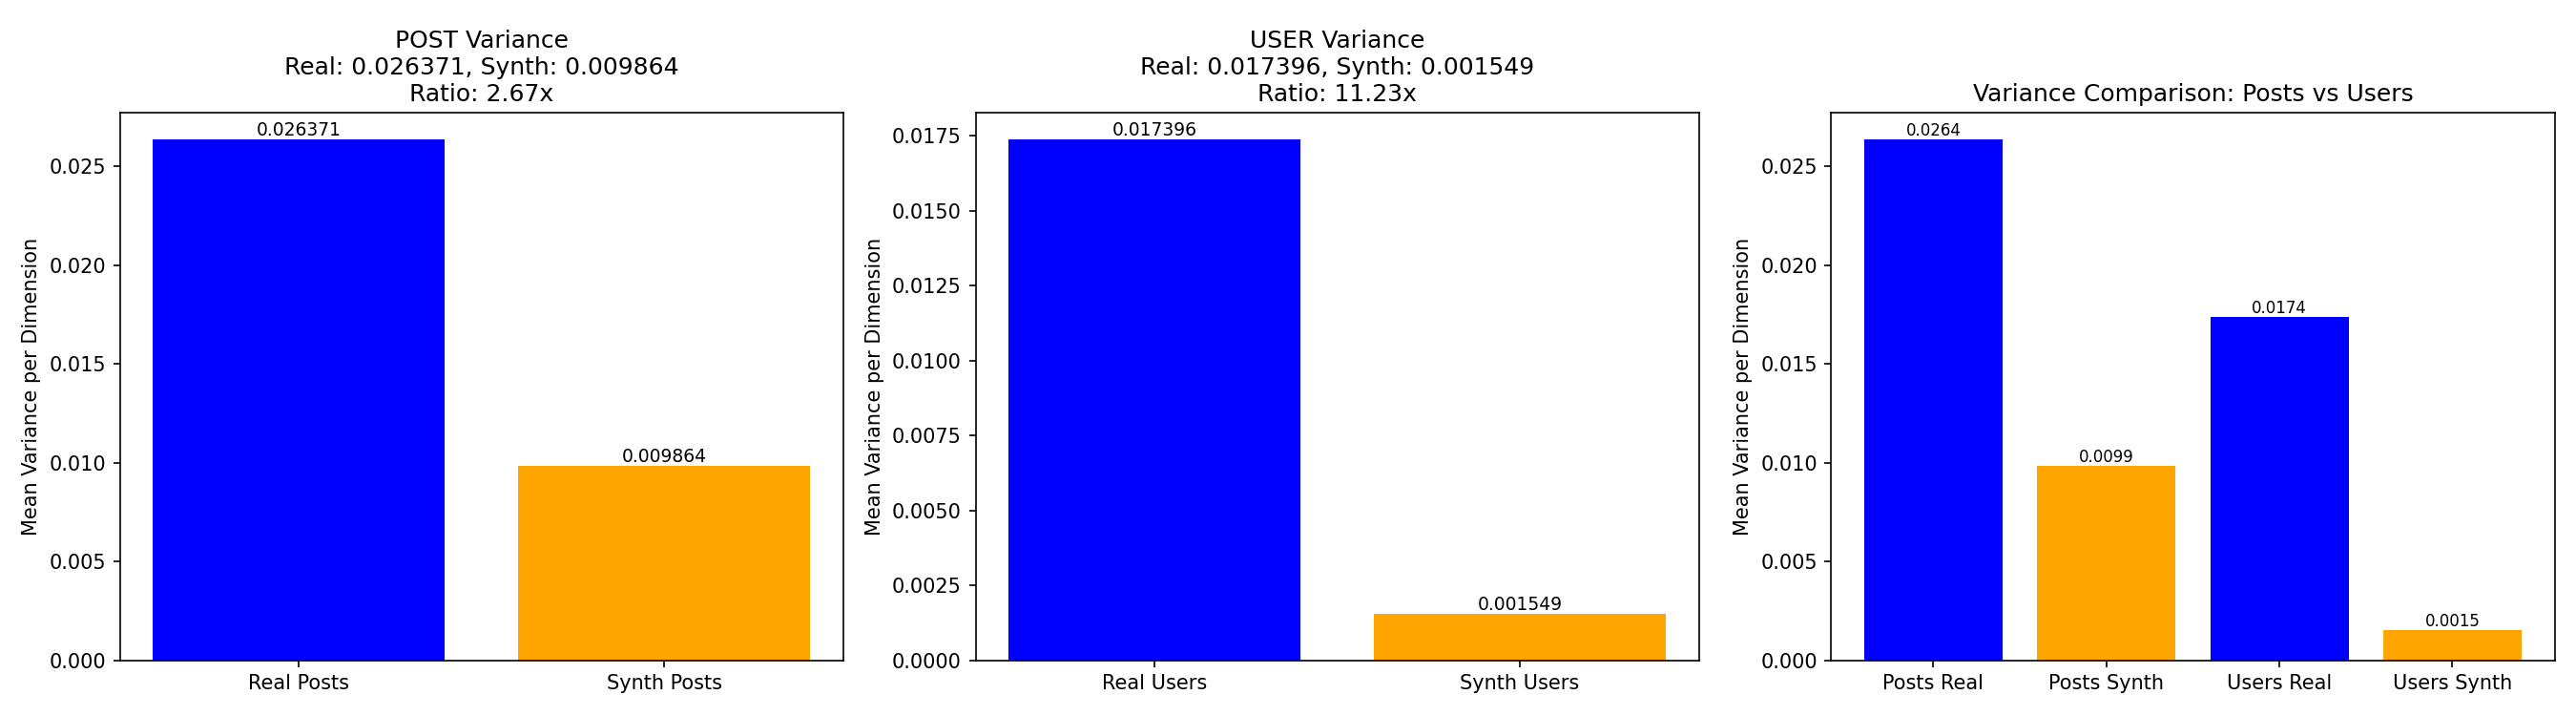
\includegraphics[width=0.95\textwidth]{figures/embedding_variance_summary.png}
% 	\caption{Variance comparison for posts and users. The left panel shows post-level variance, the center shows user-level variance, and the right panel provides a direct comparison. Synthetic data exhibits dramatically lower variance at both levels.}
% 	\label{fig:variance_summary}
% \end{figure}



\subsection*{User-Level Embedding Aggregation}

When aggregating post embeddings by user (computing the mean embedding for each user's posts), the homogeneity becomes even more pronounced. Table~\ref{tab:user_embedding_stats} presents the user-level statistics for both real and synthetic users.

\begin{table}[H]
	\centering
	\caption{User-level embedding statistics: Real vs Synthetic users}
	\label{tab:user_embedding_stats}
	\begin{tabular}{lrr}
		\toprule
		\textbf{Metric}                      & \textbf{Real}             & \textbf{Synthetic} \\
		\midrule
		Total users                          & 25583                    & 1,000              \\
		User-User cosine similarity (mean)   & 0.872                     & 0.988              \\
		User-User cosine similarity (std)    & 0.083                     & 0.004              \\
		Within-group variance (mean per dim) & 0.0174                    & 0.0015             \\
		Cross-group cosine similarity (mean) & \multicolumn{2}{c}{0.893}                      \\
		\bottomrule
	\end{tabular}
\end{table}

The cross-group cosine similarity of \textbf{0.893} indicates moderate semantic similarity between real and synthetic users. However, the within-group metrics reveal stark differences: synthetic users have a within-group cosine similarity of \textbf{0.988} with standard deviation of only 0.004, meaning they are nearly indistinguishable from each other. Real users, in contrast, show a mean similarity of \textbf{0.872} with much higher variance (std=\textbf{0.083}), reflecting natural diversity in content and interests, even though they are still relatively similar on average.

% \begin{figure}[H]
% 	\centering
% 	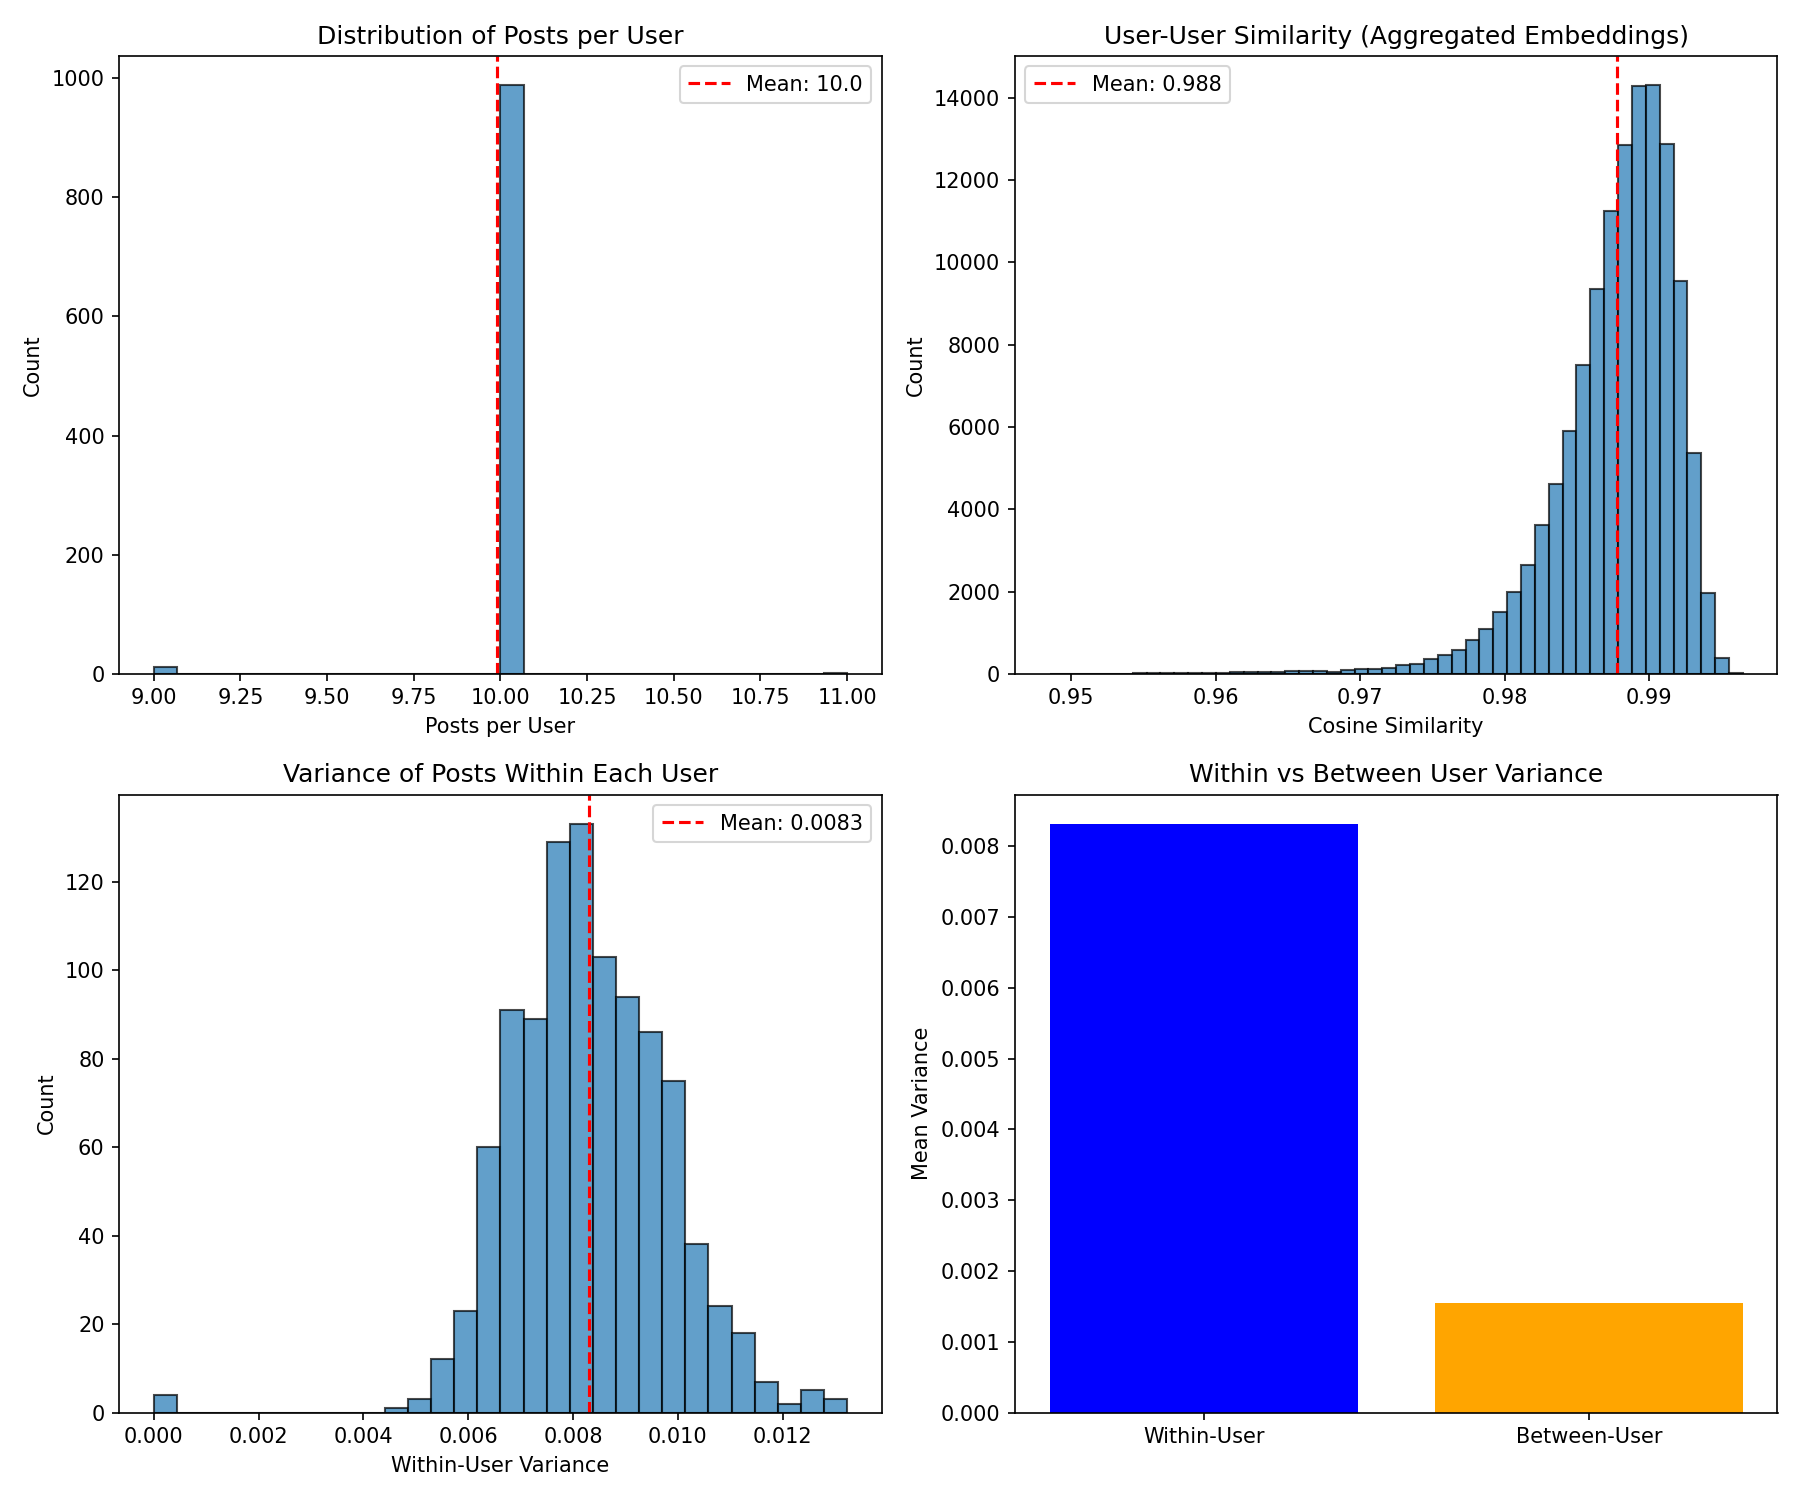
\includegraphics[width=0.9\textwidth]{figures/user_embedding_analysis.png}
% 	\caption{User embedding analysis showing the distribution of posts per user, cosine similarity between users, and variance decomposition. The extremely high user similarity (0.988) indicates synthetic users lack diversity.}
% 	\label{fig:user_embedding}
% \end{figure}

% \subsection*{Nearest Neighbors Analysis}

% To further investigate the embedding space structure, a nearest neighbors analysis was performed. Figure~\ref{fig:nearest_neighbors} shows the composition of nearest neighbors for both real and synthetic posts.

% \begin{figure}[H]
% 	\centering
% 	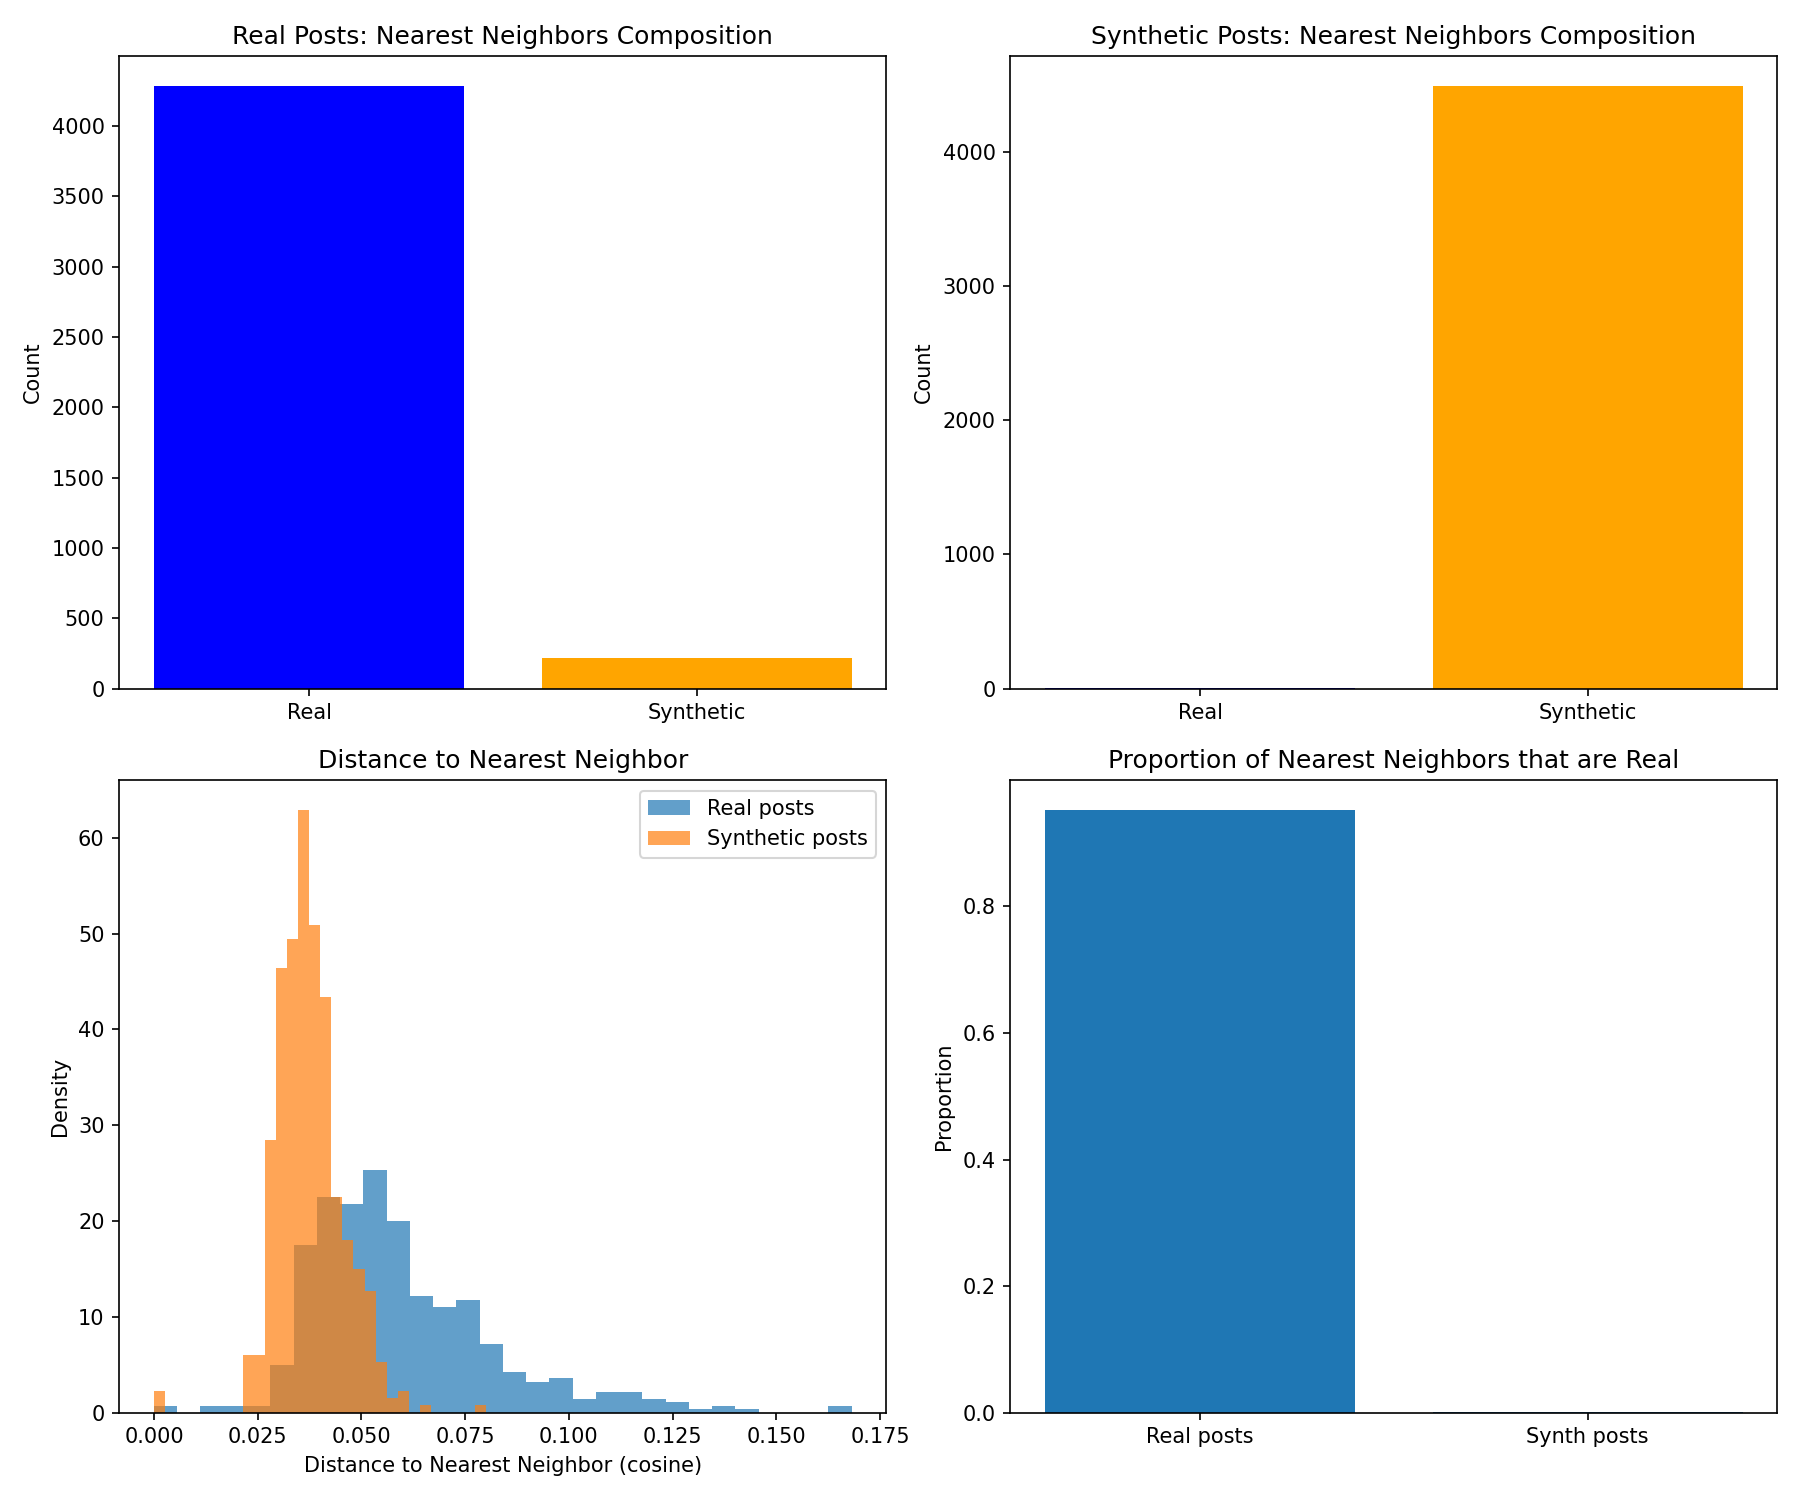
\includegraphics[width=0.9\textwidth]{figures/nearest_neighbors_analysis.png}
% 	\caption{Nearest neighbors composition: Real posts find 95\% of their neighbors among other real posts, while synthetic posts find 99.9\% of their neighbors among other synthetic posts, forming an isolated cluster.}
% 	\label{fig:nearest_neighbors}
% \end{figure}

% The analysis reveals a stark separation:
% \begin{itemize}
% 	\item \textbf{Real posts}: 95.2\% of nearest neighbors are other real posts
% 	\item \textbf{Synthetic posts}: 99.9\% of nearest neighbors are other synthetic posts
% \end{itemize}

% This confirms that synthetic posts form an isolated cluster in the embedding space, disconnected from the real data distribution. This isolation may cause issues during inference, as the model encounters out-of-distribution embeddings.

% \subsection*{Implications for Link Prediction}

% The embedding analysis reveals several challenges for the link prediction task:

% \begin{enumerate}
% 	\item \textbf{Homogeneity}: Synthetic nodes are too similar to each other, making it difficult for the model to learn meaningful distinctions
% 	\item \textbf{Isolation}: Synthetic embeddings form a separate cluster, disconnected from real embeddings
% 	\item \textbf{OOD Risk}: When predicting links involving synthetic nodes, the model operates on out-of-distribution data
% \end{enumerate}

% Potential mitigation strategies include:
% \begin{itemize}
% 	\item Regenerating synthetic posts with more diverse prompts
% 	\item Adding noise to synthetic embeddings to increase variance
% 	\item Connecting synthetic nodes to real nodes in the graph structure
% 	\item Using higher probability thresholds (0.7-0.8) for filtering predictions
% \end{itemize}


% \section{Summary}

% The data understanding phase revealed a rich dataset of 182,545 posts from the Gab social network, spanning nearly a decade (2016-2025). Key findings include:

% \begin{itemize}
% 	\item \textbf{Growth pattern}: The platform shows exponential growth, with 2025 data alone representing 68\% of all posts
% 	\item \textbf{Language homogeneity}: 97\% English content, making it suitable for single-language NLP tasks
% 	\item \textbf{Content characteristics}: Short-form content dominates (median 89 characters, 13 words) with heavy-tailed distributions
% 	\item \textbf{Engagement patterns}: Highly skewed distributions with 28\% zero-engagement posts and viral outliers reaching 20,000+ interactions
% 	\item \textbf{User dynamics}: Power-law distribution with 0.43\% of users (116 power users) driving significant content volume
% 	\item \textbf{Data quality}: High completeness (99.52\%) with only the \texttt{language} field showing missing values; perfect snapshot-incremental consistency
% 	\item \textbf{Duplicate trend}: Increasing content duplication over time (from 1.79\% to 10.04\%), suggesting potential bot activity or viral content resharing
% 	\item \textbf{Embedding quality}: Synthetic embeddings show extreme homogeneity (cosine sim 0.925 vs 0.821 for real) and form an isolated cluster, posing challenges for link prediction
% \end{itemize}

% The dataset is well-suited for link prediction and social network analysis tasks, with the temporal snapshots enabling longitudinal studies of network evolution. The preprocessing pipeline should address the minor missing values, consider strategies for handling the heavy-tailed engagement distributions, and account for the embedding homogeneity in synthetic data.

\titleformat{\chapter}[hang]{\Huge\bfseries}{\selectfont \thechapter\hsp\textcolor{red}{\emoji{package}}\hsp}{0pt}{\Huge\bfseries}

\chapter{Data Preparation}

This chapter covers the data preparation phase of the CRISP-DM methodology.

\section{Select Data}
Select the relevant data for the analysis.

% \subsection{Sampling}
% Apply sampling techniques to create representative subsets.

% \subsection{Feature Selection}
% Select the most relevant features for the analysis.

\section{Clean Data}
Clean the data by handling missing values, outliers, and errors.

\section{Construct Data}
Construct new features or transform existing ones.

\section{Integrate Data}
Integrate data from multiple sources.

\section{Format Data}
Format the data according to the requirements of the modeling tools.
\titleformat{\chapter}[hang]{\Huge\bfseries}{\selectfont \thechapter\hsp\textcolor{red}{\emoji{abacus}}\hsp}{0pt}{\Huge\bfseries}

\chapter{Modeling}

This chapter covers the modeling phase of the CRISP-DM methodology.

% Add your content here for modeling

\section{Select Modeling Techniques}

For dynamic graph analysis, we selected \textbf{EvolveGCN} (Evolving Graph Convolutional Networks) \cite{parejaEvolveGCNEvolvingGraph2020} as our primary modeling approach. This technique addresses a critical limitation of existing methods: the requirement for nodes to be present throughout the entire time span (training and testing), making them less applicable when node sets frequently change or completely differ between time steps.

\subsection*{Motivation and Context}

Traditional graph neural network approaches for dynamic graphs typically resort to node embeddings and use recurrent neural networks to regulate these embeddings and learn temporal dynamics. However, this approach faces significant challenges in practical scenarios where:

\begin{itemize}
    \item New nodes emerge after training
    \item Nodes frequently appear and disappear
    \item Node sets at different time steps may completely differ
\end{itemize}

EvolveGCN resolves these challenges by focusing on model adaptation rather than node embeddings. Instead of using RNNs to learn dynamics from node features extracted by GNNs, EvolveGCN uses RNNs to regulate the GCN model (network parameters) at every time step \cite{parejaEvolveGCNEvolvingGraph2020}. This approach effectively performs model adaptation without requiring nodes to be present throughout the entire time span, making it suitable for our social network analysis where users may join or leave the platform.

\subsection*{Architecture Overview}

EvolveGCN adapts the Graph Convolutional Network (GCN) model along the temporal dimension without resorting to node embeddings. The proposed approach captures the dynamism of the graph sequence through using an RNN to evolve the GCN parameters, with two architectures considered for parameter evolution \cite{parejaEvolveGCNEvolvingGraph2020}.

At each time step $t$, the input data consists of the pair $(A_t \in \mathbb{R}^{n \times n}, X_t \in \mathbb{R}^{n \times d})$, where $A_t$ is the graph adjacency matrix and $X_t$ is the matrix of node features (each row is a $d$-dimensional feature vector).

\subsection*{Graph Convolution Layer}

A GCN consists of multiple layers of graph convolution, which is similar to a perceptron but additionally has a neighborhood aggregation step motivated by spectral convolution. At time $t$, the $l$-th layer takes the adjacency matrix $A_t$ and the node embedding matrix $H_t^{(l)}$ as input, and uses a weight matrix $W_t^{(l)}$ to update the node embedding matrix to $H_t^{(l+1)}$ as output:

\begin{equation}
H_t^{(l+1)} = \text{GCONV}(A_t, H_t^{(l)}, W_t^{(l)}) := \sigma(\hat{A}_t H_t^{(l)} W_t^{(l)})
\end{equation}

where $\hat{A}_t$ is a normalization of $A_t$ defined as:

\begin{equation}
\hat{A} = \tilde{D}^{-\frac{1}{2}} \tilde{A} \tilde{D}^{-\frac{1}{2}}, \quad \tilde{A} = A + I, \quad \tilde{D} = \text{diag}\left(\sum_j \tilde{A}_{ij}\right)
\end{equation}

and $\sigma$ is the activation function (typically ReLU) for all but the output layer. The initial embedding matrix comes from the node features: $H_t^{(0)} = X_t$. For a GCN with $L$ layers, the output layer function $\sigma$ may be the identity (producing high-level node representations) or softmax (for node classification probabilities).

\subsection*{Weight Evolution Mechanisms}

At the heart of the proposed method is the update of the weight matrix $W_t^{(l)}$ at time $t$ based on current as well as historical information. This requirement can be naturally fulfilled by using a recurrent architecture, with two options.

\paragraph{EvolveGCN-H (Hidden State Version):} The first option treats $W_t^{(l)}$ as the hidden state of the dynamical system. A Gated Recurrent Unit (GRU) is used to update the hidden state upon time-$t$ input to the system, where the input information is naturally the node embeddings $H_t^{(l)}$:

\begin{equation}
W_t^{(l)} = \text{GRU}(H_t^{(l)}, W_{t-1}^{(l)})
\end{equation}

The implementation requires two extensions from standard GRU: (a) extending inputs and hidden states from vectors to matrices (because the hidden state is now the GCN weight matrices), and (b) matching the column dimension of the input with that of the hidden state. This is achieved through a summarization function that condenses the node embedding matrix $H_t^{(l)}$ into a matrix with appropriate dimensions using a learned parameter vector to compute weights for the rows, selecting the top-$k$ weighted rows.

\paragraph{EvolveGCN-O (Output Version):} The second option treats $W_t^{(l)}$ as the output of the dynamical system (which becomes the input at the subsequent time step). A Long Short-Term Memory (LSTM) cell models this input-output relationship, maintaining system information through a cell context that acts like the hidden state of a GRU:

\begin{equation}
W_t^{(l)} = \text{LSTM}(W_{t-1}^{(l)})
\end{equation}

In this version, node embeddings are not used at all. Implementing the -O version requires only a straightforward extension of the standard LSTM from the vector version to the matrix version.

\subsection*{Evolving Graph Convolution Unit (EGCU)}

Combining the graph convolution unit GCONV and a recurrent architecture, we reach the Evolving Graph Convolution Unit (EGCU). Depending on the way GCN weights are evolved, we have two versions:

For EvolveGCN-H:
\begin{align}
W_t^{(l)} &= \text{GRU}(H_t^{(l)}, W_{t-1}^{(l)}) \\
H_t^{(l+1)} &= \text{GCONV}(A_t, H_t^{(l)}, W_t^{(l)})
\end{align}

For EvolveGCN-O:
\begin{align}
W_t^{(l)} &= \text{LSTM}(W_{t-1}^{(l)}) \\
H_t^{(l+1)} &= \text{GCONV}(A_t, H_t^{(l)}, W_t^{(l)})
\end{align}

In the -H version, the GCN weights are treated as hidden states of the recurrent architecture; in the -O version, these weights are treated as input/outputs. Chaining the units bottom-up creates a GCN with multiple layers for one time step, and unrolling over time horizontally forms a lattice on which information ($H_t^{(l)}$ and $W_t^{(l)}$) flows.

\section{Generate Test Design} 

\section{Build Model} 

\section{Assess Model}
\titleformat{\chapter}[hang]{\Huge\bfseries}{\selectfont \thechapter\hsp\textcolor{red}{\emoji{1234}}\hsp}{0pt}{\Huge\bfseries}


\chapter{Evaluation}

This chapter covers the evaluation phase of the CRISP-DM methodology, assessing whether the developed models meet the business success criteria defined in Section~\ref{sec:business_success}.

\section{Assess Model}

The experimental configurations reported in the previous chapter were evaluated on the \texttt{Jul 2025} snapshot. Table~\ref{tab:results_comparison} presents the results, while Table~\ref{tab:class_metrics_comparison} shows per-class metrics.

\begin{table}[h]
	\centering
	\caption{Test metrics comparison: Incremental vs. Original implementation}
	\label{tab:results_comparison}
	\small
	\begin{tabular}{llccccccc}
		\toprule
		 &  & \textbf{LR} & \textbf{NM} & \textbf{MAP} & \textbf{AUC} & \textbf{Mac P} & \textbf{Mac R} & \textbf{Mac F1} \\
		\midrule
		\multirow{4}{*}{\rotatebox{90}{\textbf{Incr.}}}
		 &  & 0.001       & 1           & 0.78       & 0.78       & 0.25         & 0.49         & 0.33          \\
		 &  & 0.001       & 2           & 0.64       & 0.74       & 0.75         & 0.68         & 0.69          \\
		 &  & 0.0005      & 1           & 0.78       & 0.80       & 0.68         & 0.52         & 0.38          \\
		 &  & 0.0005      & 2           & 0.62       & 0.72       & 0.73         & 0.68         & 0.69 \\
		\midrule
		\multirow{4}{*}{\rotatebox{90}{\textbf{Orig.}}}
		 &  & 0.001       & 1           & 0.87       & 0.63       & 0.86         & 0.86         & 0.86          \\
		 &  & 0.001       & 2           & 0.77       & 0.65       & 0.82         & 0.83         & 0.83          \\
		 &  & 0.0005      & 1           & 0.86       & 0.64       & 0.82         & 0.79         & 0.78          \\
		 &  & 0.0005      & 2           & 0.76       & 0.65       & 0.81         & 0.84         & 0.81          \\
		\bottomrule
	\end{tabular}

	\vspace{0.5em}
	\footnotesize
	\textit{Incr. = Incremental, Orig. = Original, LR = Learning Rate, NM = Negative Multiplier, Mac P = Macro Precision, Mac R = Macro Recall}
\end{table}



\begin{table}[h]
	\centering
	\caption{Per-class metrics comparison: Incremental vs. Original implementation}
	\label{tab:class_metrics_comparison}
	\small
	\begin{tabular}{llcccccccc}
		\toprule
		 &  & \textbf{LR} & \textbf{NM} & \multicolumn{3}{c}{\textbf{Class 0 (Non-link)}} & \multicolumn{3}{c}{\textbf{Class 1 (Link)}}                             \\
		\cmidrule(lr){5-7} \cmidrule(lr){8-10}
		 &  &             &             & P                                               & R                                           & F1   & P    & R    & F1   \\
		\midrule
		\multirow{4}{*}{\rotatebox{90}{\textbf{Incr.}}}
		 &  & 0.001       & 1           & 0.00                                            & 0.00                                        & 0.00 & 0.49 & 0.97 & 0.65 \\
		 &  & 0.001       & 2           & 0.77                                            & 0.92                                        & 0.83 & 0.73 & 0.44 & 0.55 \\
		 &  & 0.0005      & 1           & 0.85                                            & 0.04                                        & 0.08 & 0.51 & 0.99 & 0.67 \\
		 &  & 0.0005      & 2           & 0.77                                            & 0.90                                        & 0.83 & 0.69 & 0.47 & 0.56 \\
		\midrule
		\multirow{4}{*}{\rotatebox{90}{\textbf{Orig.}}}
		 &  & 0.001       & 1           & 0.89                                            & 0.83                                        & 0.86 & 0.84 & 0.89 & 0.87 \\
		 &  & 0.001       & 2           & 0.89                                            & 0.88                                        & 0.88 & 0.76 & 0.78 & 0.77 \\
		 &  & 0.0005      & 1           & 0.93                                            & 0.62                                        & 0.74 & 0.71 & 0.96 & 0.82 \\
		 &  & 0.0005      & 2           & 0.95                                            & 0.76                                        & 0.84 & 0.66 & 0.93 & 0.77 \\
		\bottomrule
	\end{tabular}

	\vspace{0.5em}
	\footnotesize
	\textit{Incr. = Incremental, Orig. = Original, LR = Learning Rate, NM = Negative Multiplier, P = Precision, R = Recall}
\end{table}

\paragraph{Overall Performance Comparison.} The Original implementation achieves significantly higher MAP (0.87 vs. 0.78) and Macro F1 (0.86 vs. 0.69), indicating superior ranking quality and classification performance. However, the Incremental approach achieves notably higher AUC (0.80 vs. 0.65), suggesting better discrimination ability at various probability thresholds.

\paragraph{Choosing MAP as discriminative metric.} Choosing MAP as the primary metric for model selection is justified by its focus on ranking quality, which is critical for link prediction tasks. However, as we can see in the first configuration of the Incremental approach, the best model predicts always 1, in practice the model is not able to discriminate between the two classes.

\paragraph{Negative Sampling Multiplier Impact.} For both approaches, increasing NM from 1 to 2, it reduces MAP (Incremental: 0.78 $\rightarrow$ 0.64; Original: 0.87 $\rightarrow$ 0.77), as expected. However, it improves AUC (Incremental: 0.78 $\rightarrow$ 0.72; Original: 0.63 $\rightarrow$ 0.65), suggesting that a higher proportion of negative samples helps the model learn better decision boundaries, albeit at the cost of ranking quality.

\paragraph{Learning Rate Impact.} The learning rate shows different effects across approaches:
\begin{itemize}
	\item \textbf{Incremental}: LR=0.0005 achieves higher AUC (0.8037) but with worse class balance
	\item \textbf{Original}: LR=0.001 consistently outperforms LR=0.0005 across all metrics
\end{itemize}

In general, the original approach demonstrates stronger performance in terms of MAP and Macro F1.

% \subsection*{Limitations and Threats to Validity}

% Several factors may affect the generalizability of results:

% \begin{itemize}
% 	\item \textbf{Dataset Specificity}: Results on Gab may not transfer to other social platforms with different user demographics or content moderation policies.

% 	\item \textbf{Temporal Coverage}: The dataset spans 2016-2025, but platform dynamics may have changed significantly over this period.

% 	\item \textbf{Feature Limitations}: BERT embeddings capture semantic content but may miss important signals from user metadata, temporal patterns, or external events.

% 	\item \textbf{Evaluation Bias}: The cumulative edge assumption (edges persist once created) simplifies the task but may not reflect real-world unfollowing behavior.
% \end{itemize}

\subsection*{Graph Metrics Analysis}

Table~\ref{tab:graph_metrics} presents the comparison across degree, modularity, average path length, and clustering coefficient. We report only the metrics computed on graph where it's worth to: infact, some configuration tends to always assign the same label to all the edges, so the resulting graph is either a complete graph or an empty graph, and in both cases the metrics are not meaningful. For the first case (complete graph), this can be due to the training process not converging properly, while for the second case (empty graph) this can be due to a lack of generalization of the model, or from the nature of the real and synthetic data that, as analyzed in the previous chapters, are clustered in different part of the space.

\begin{table}[h]
	\centering
	\caption{Graph metrics comparison: Real vs. Synthetic Networks}
	\label{tab:graph_metrics}
	\begin{tabular}{lccccc}
		\toprule
		\textbf{Network}        & \textbf{Avg Degree} & \textbf{Modularity} & \textbf{Avg Path} & \textbf{Clustering Coeff.} \\
		\midrule
		Facebook                & 43.69               & 0.8348              & 3.6167            & 0.6055                     \\
		Twitter                 & 21.75               & 0.8042              & 4.9044            & 0.5653                     \\
		Google+\footnotemark[4] & 127.06              & 0.4742              & 3.3163            & 0.4901                     \\
		Gab (Ours)              & 32.11               & 0.2742              & 3.0384           & 0.0808                     \\
		\midrule
		Incr., LR=0.0005, NM=1  & 220.35              & -0.0013             & 1.0167            & 0.5941                     \\
		\bottomrule
	\end{tabular}
\end{table}

\footnotetext[4]{Due to the dimension of the Google+ dataset, we report the metrics for the largest connected component (LCC) considering the 20\% of nodes with the highest degree.}

\subsubsection*{Analysis of Synthetic Networks}

The synthetic network generated by the Incremental configuration (LR=0.0005, NM=1) exhibits significant structural differences compared to real social networks:

\paragraph{Degree Distribution.} The synthetic network shows an extremely high average degree (220.35), approximately 7$\times$ higher than the Gab dataset (32.11) and 5$\times$ higher than Google+ (127.06). This indicates that the model tends to predict edges too liberally, creating an overly dense network.
% In real social networks, users typically maintain a limited number of connections due to cognitive constraints and social capital limitations, resulting in sparse graph structures.

\paragraph{Community Structure.} The near-zero modularity (-0.0013) indicates a complete absence of community structure. Real social networks typically exhibit modularity values between 0.3 and 0.8, reflecting the natural tendency of users to form groups.
%The synthetic network's lack of modularity suggests that the model does not capture the homophilic patterns that drive real social network formation.

\paragraph{Small-World Property.} The average path length of 1.0167 is unrealistically low compared to real networks (3.0-4.9). This is a direct consequence of the high density: in a nearly complete graph, most nodes are directly connected or separated by only one intermediate node. Real social networks maintain the ``small-world'' property with moderate path lengths (typically 3-6) while remaining sparse.

\paragraph{Clustering Coefficient.} Interestingly, the clustering coefficient (0.5941) falls within the range of real social networks (0.49-0.61). This suggests that when the model does predict edges, it tends to close triangles. However, this metric is somewhat misleading given the extreme density of the network.

\subsubsection*{GCN Embedding Visualization}

To better understand the behaviors of our model, we visualized the GCN embeddings using PCA and t-SNE dimensionality reduction. Figures~\ref{fig:gcn_original} and~\ref{fig:gcn_incremental} present the embeddings for the Original and Incremental configurations, showing the distribution of real users (blue) and synthetic users (red) in the learned embedding space.

\begin{figure}[H]
	\centering
	\begin{subfigure}[b]{0.48\textwidth}
		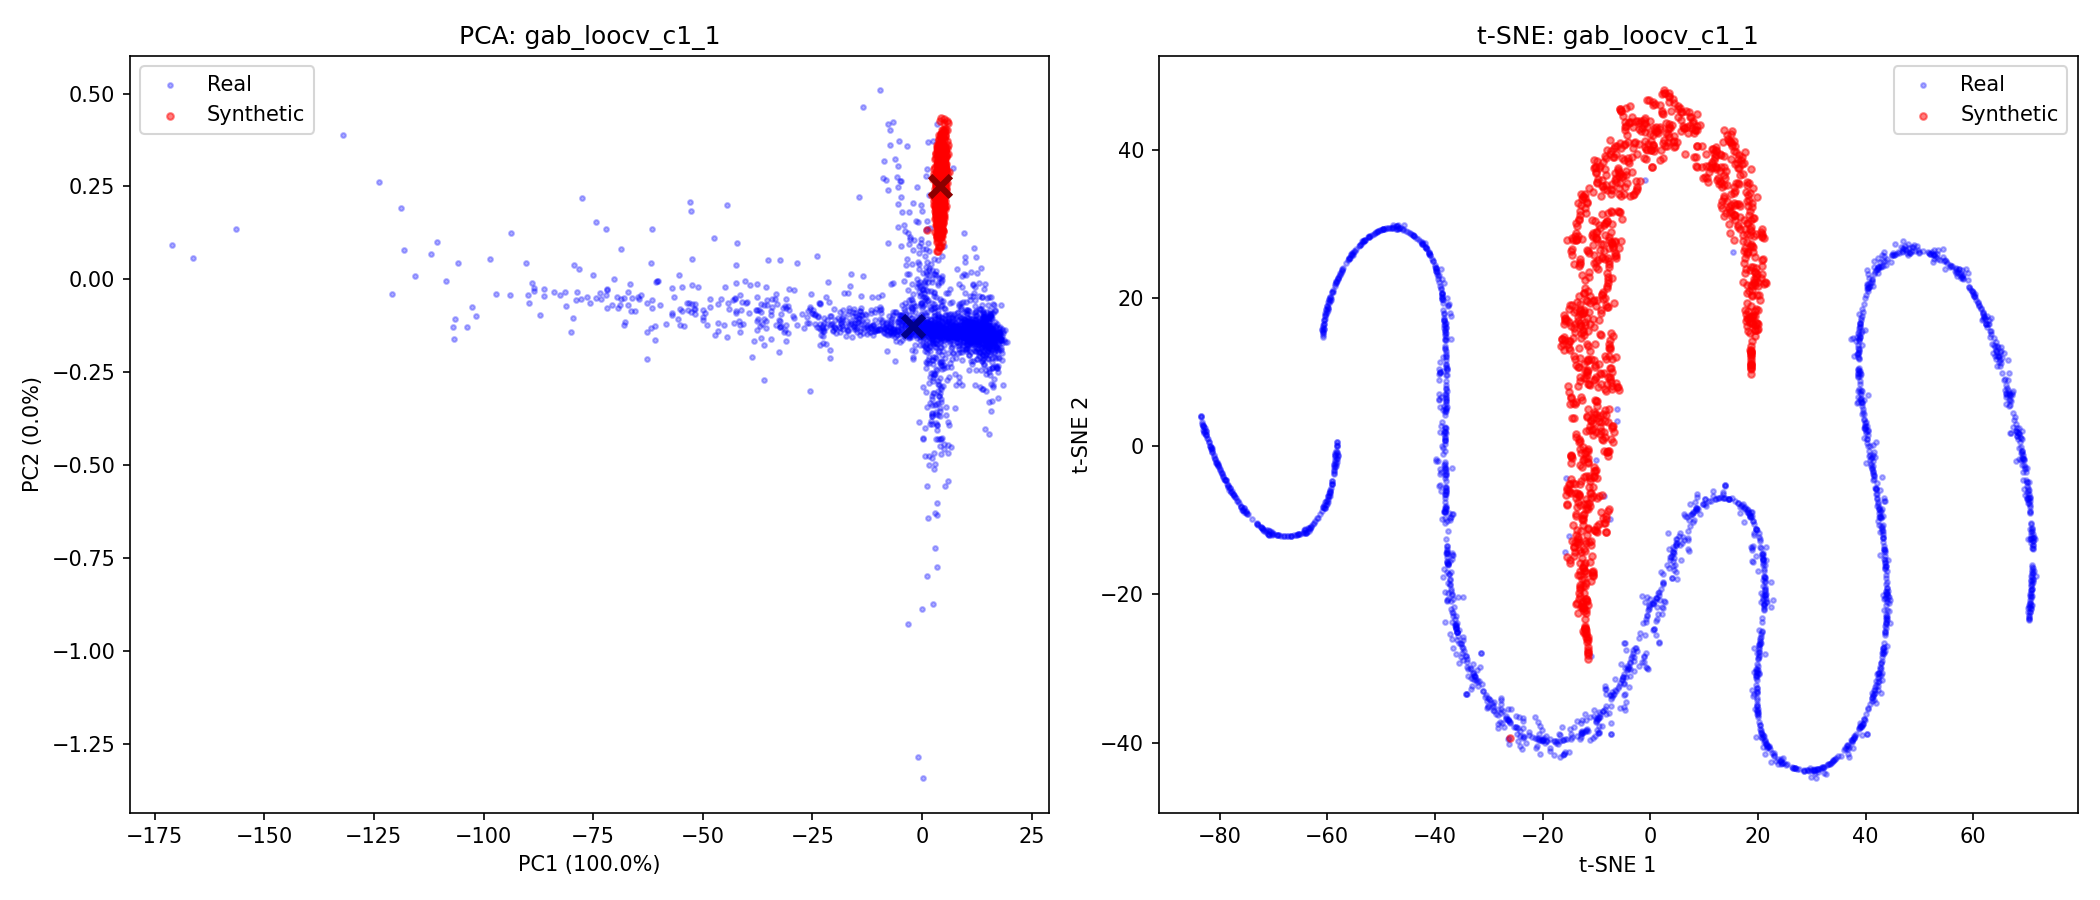
\includegraphics[width=\textwidth]{figures/gab_loocv_c1_1_gcn_visualization.png}
		\caption{Config 1, NM=1 (LR=0.001)}
	\end{subfigure}
	\hfill
	\begin{subfigure}[b]{0.48\textwidth}
		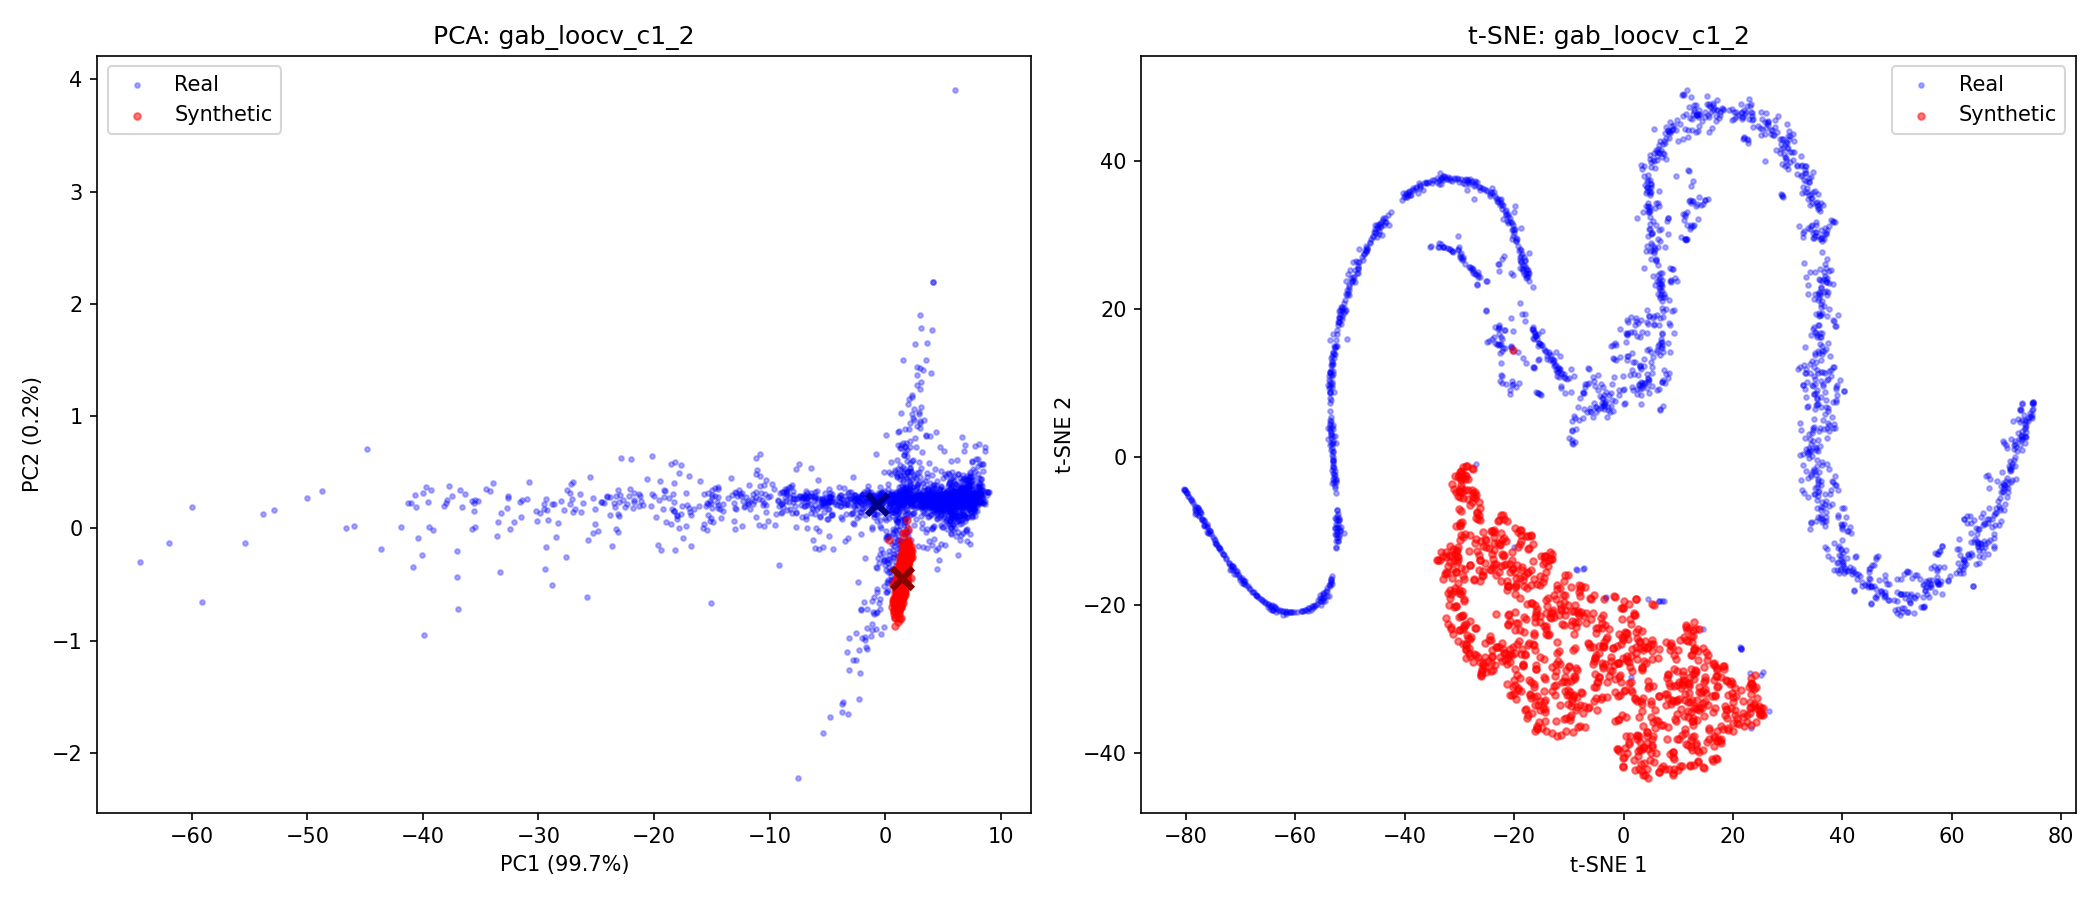
\includegraphics[width=\textwidth]{figures/gab_loocv_c1_2_gcn_visualization.png}
		\caption{Config 1, NM=2 (LR=0.001)}
	\end{subfigure}

	\vspace{0.5em}

	\begin{subfigure}[b]{0.48\textwidth}
		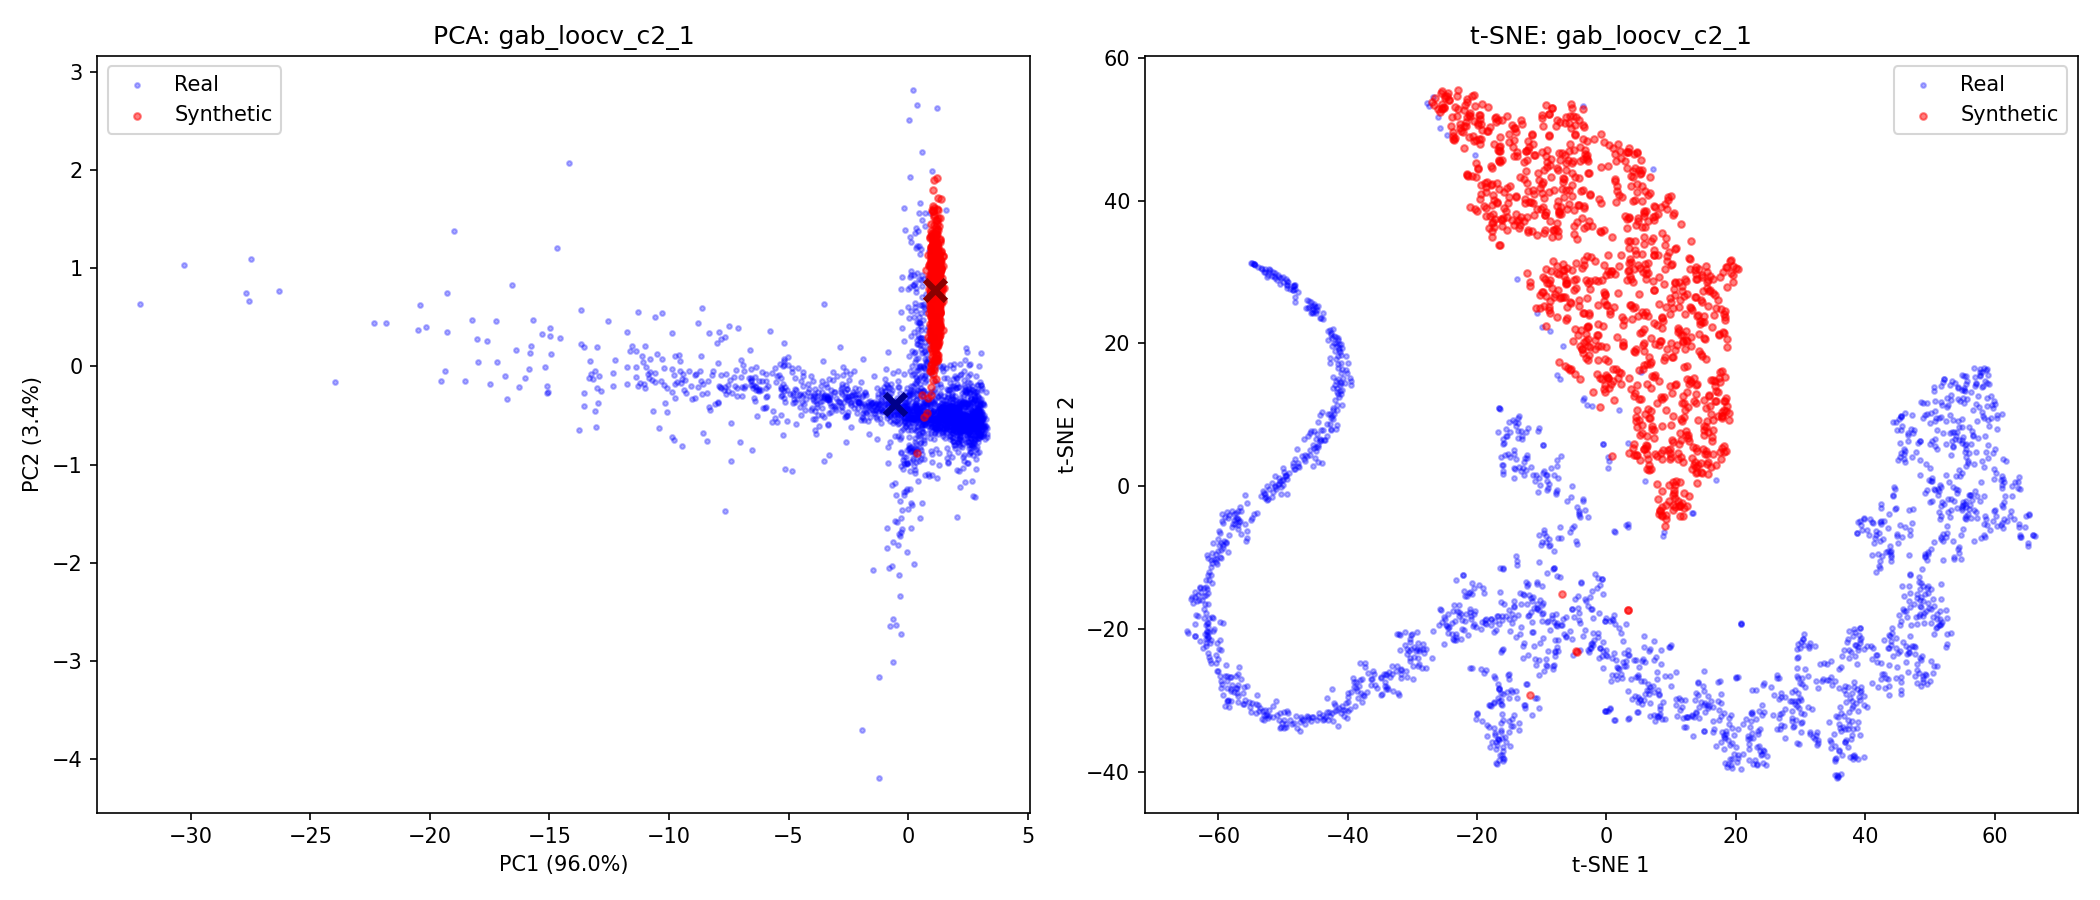
\includegraphics[width=\textwidth]{figures/gab_loocv_c2_1_gcn_visualization.png}
		\caption{Config 2, NM=1 (LR=0.0005)}
	\end{subfigure}
	\hfill
	\begin{subfigure}[b]{0.48\textwidth}
		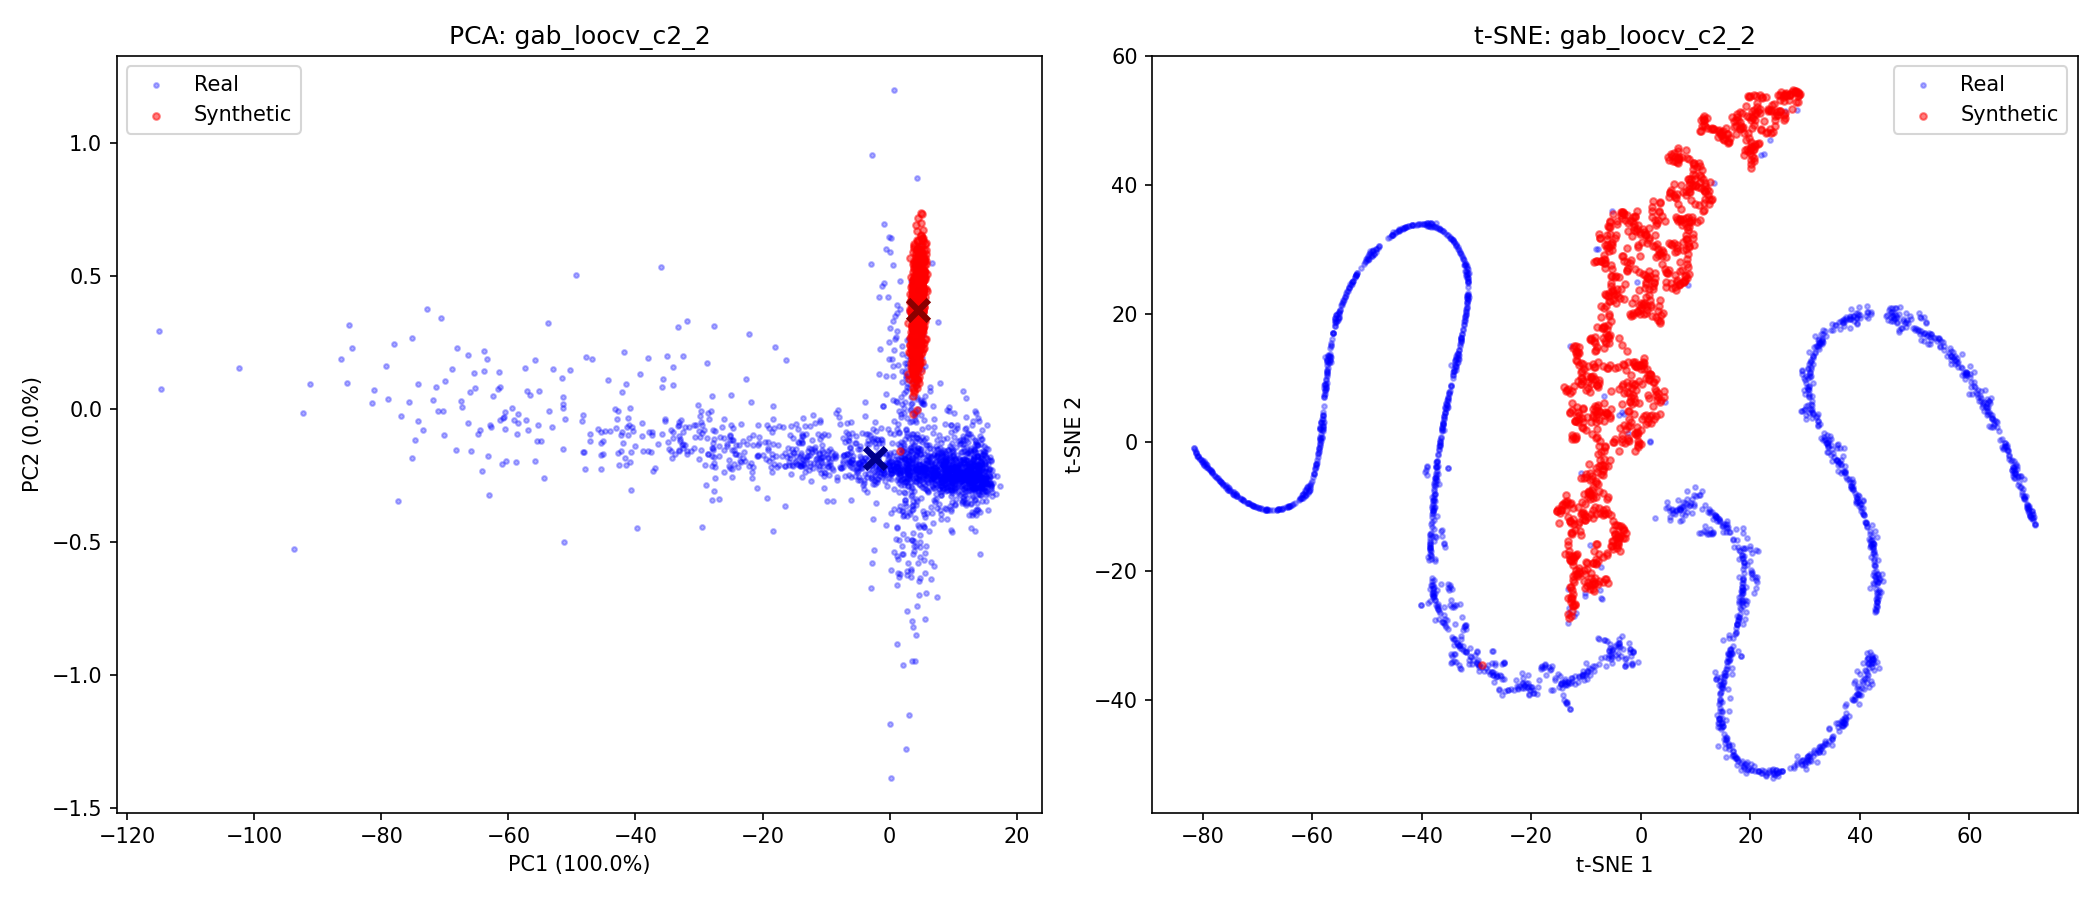
\includegraphics[width=\textwidth]{figures/gab_loocv_c2_2_gcn_visualization.png}
		\caption{Config 2, NM=2 (LR=0.0005)}
	\end{subfigure}
	\caption{PCA and t-SNE visualization of GCN embeddings for Original implementation. Blue points represent real users, red points represent synthetic users.}
	\label{fig:gcn_original}
\end{figure}

\begin{figure}[H]
	\centering
	\begin{subfigure}[b]{0.48\textwidth}
		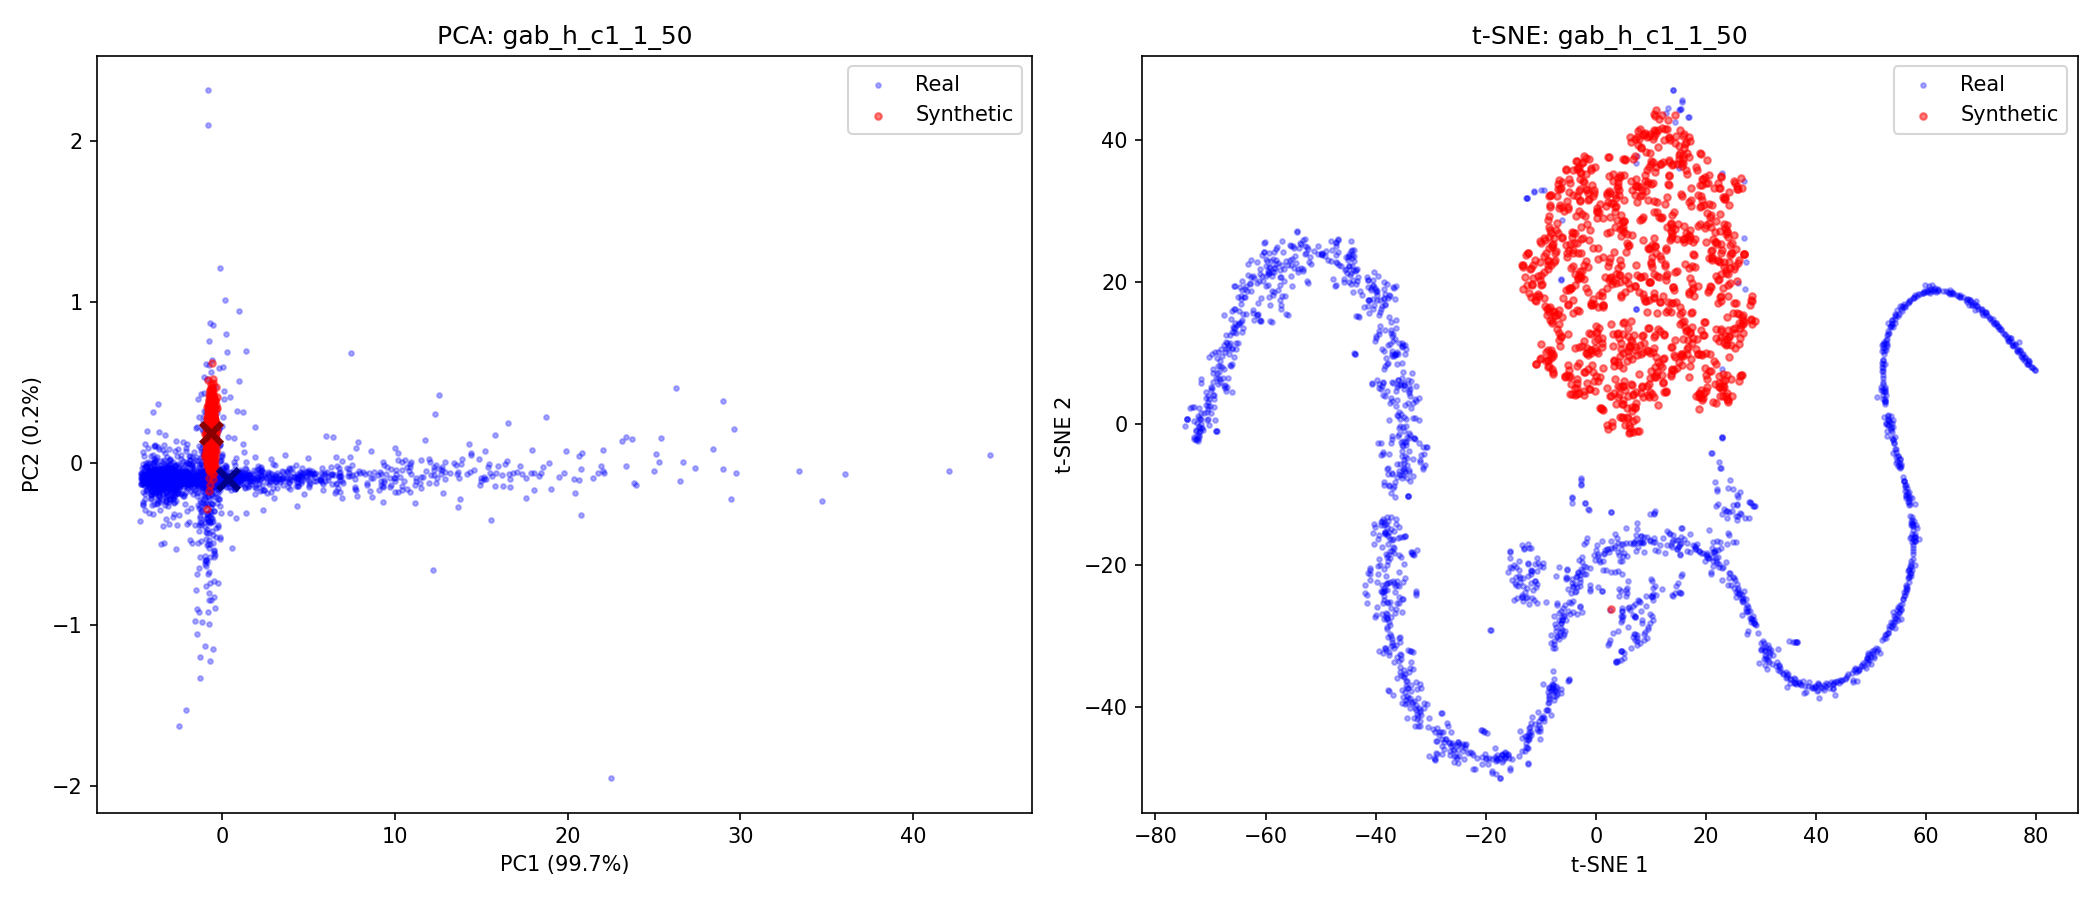
\includegraphics[width=\textwidth]{figures/gab_h_c1_1_50_gcn_visualization.png}
		\caption{Config 1, NM=1 (LR=0.001)}
	\end{subfigure}
	\hfill
	\begin{subfigure}[b]{0.48\textwidth}
		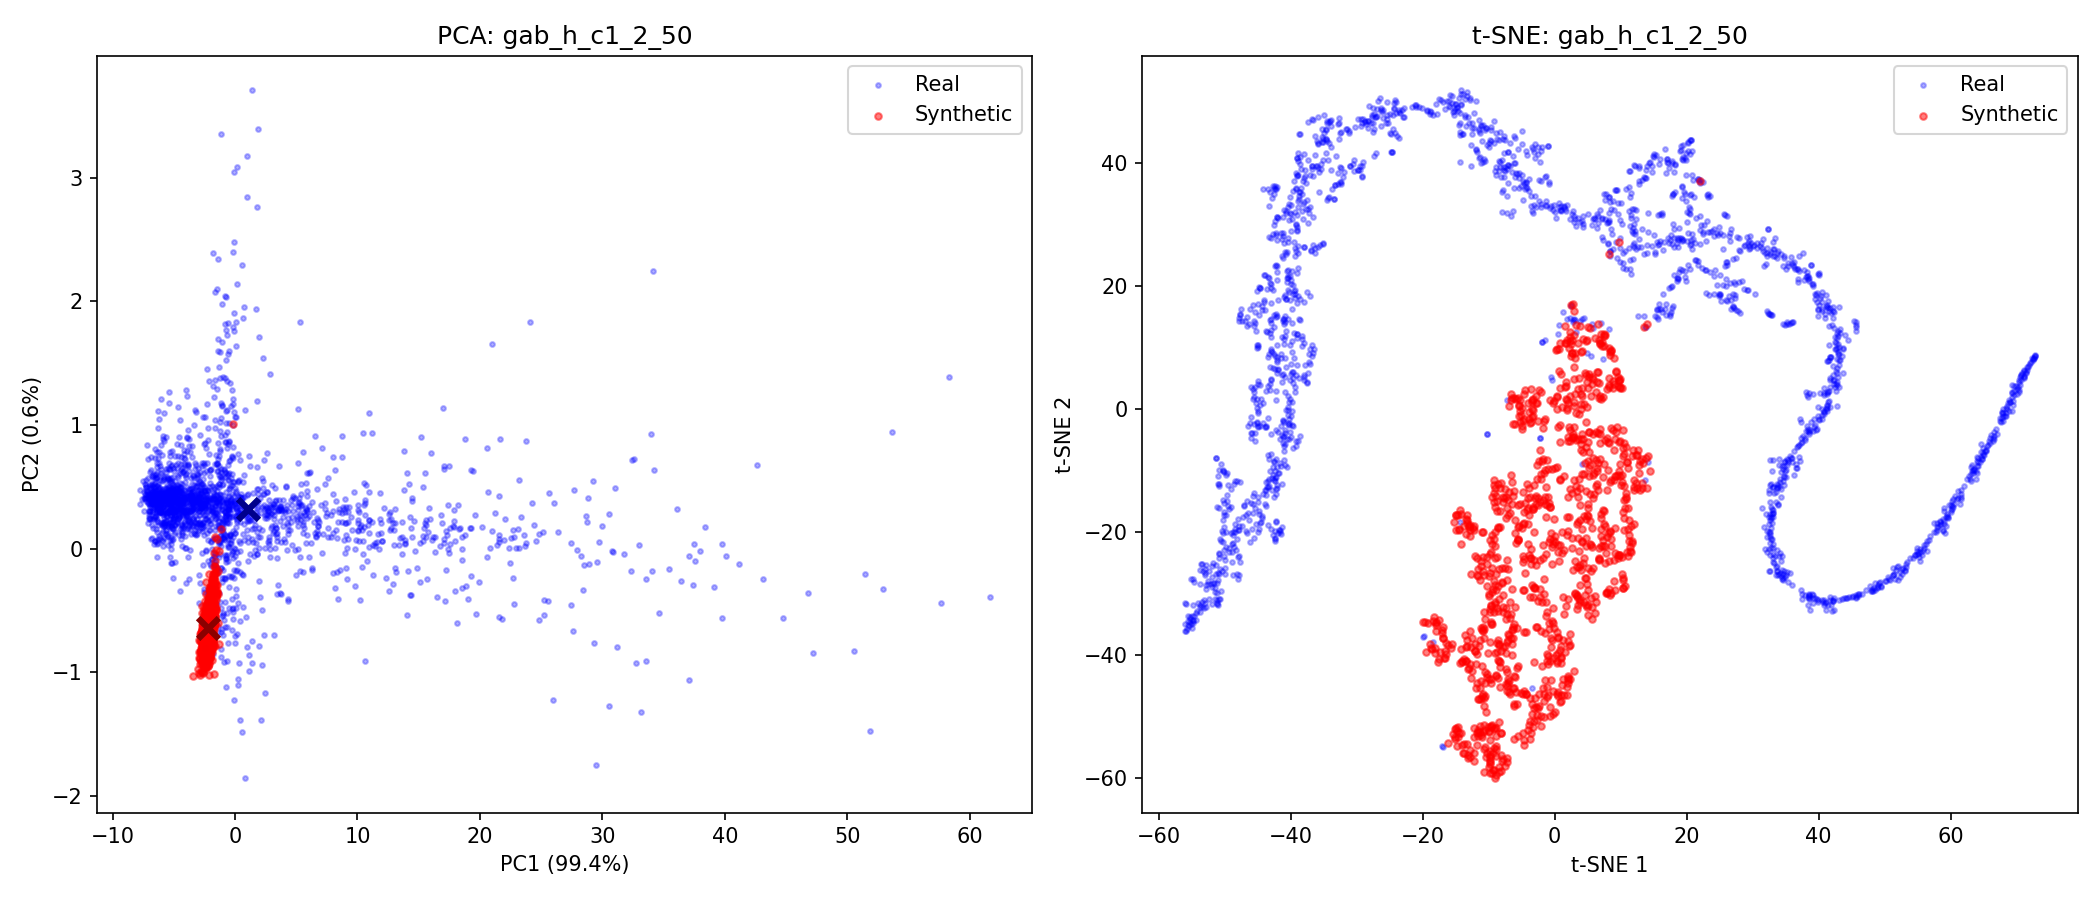
\includegraphics[width=\textwidth]{figures/gab_h_c1_2_50_gcn_visualization.png}
		\caption{Config 1, NM=2 (LR=0.001)}
	\end{subfigure}

	\vspace{0.5em}

	\begin{subfigure}[b]{0.48\textwidth}
		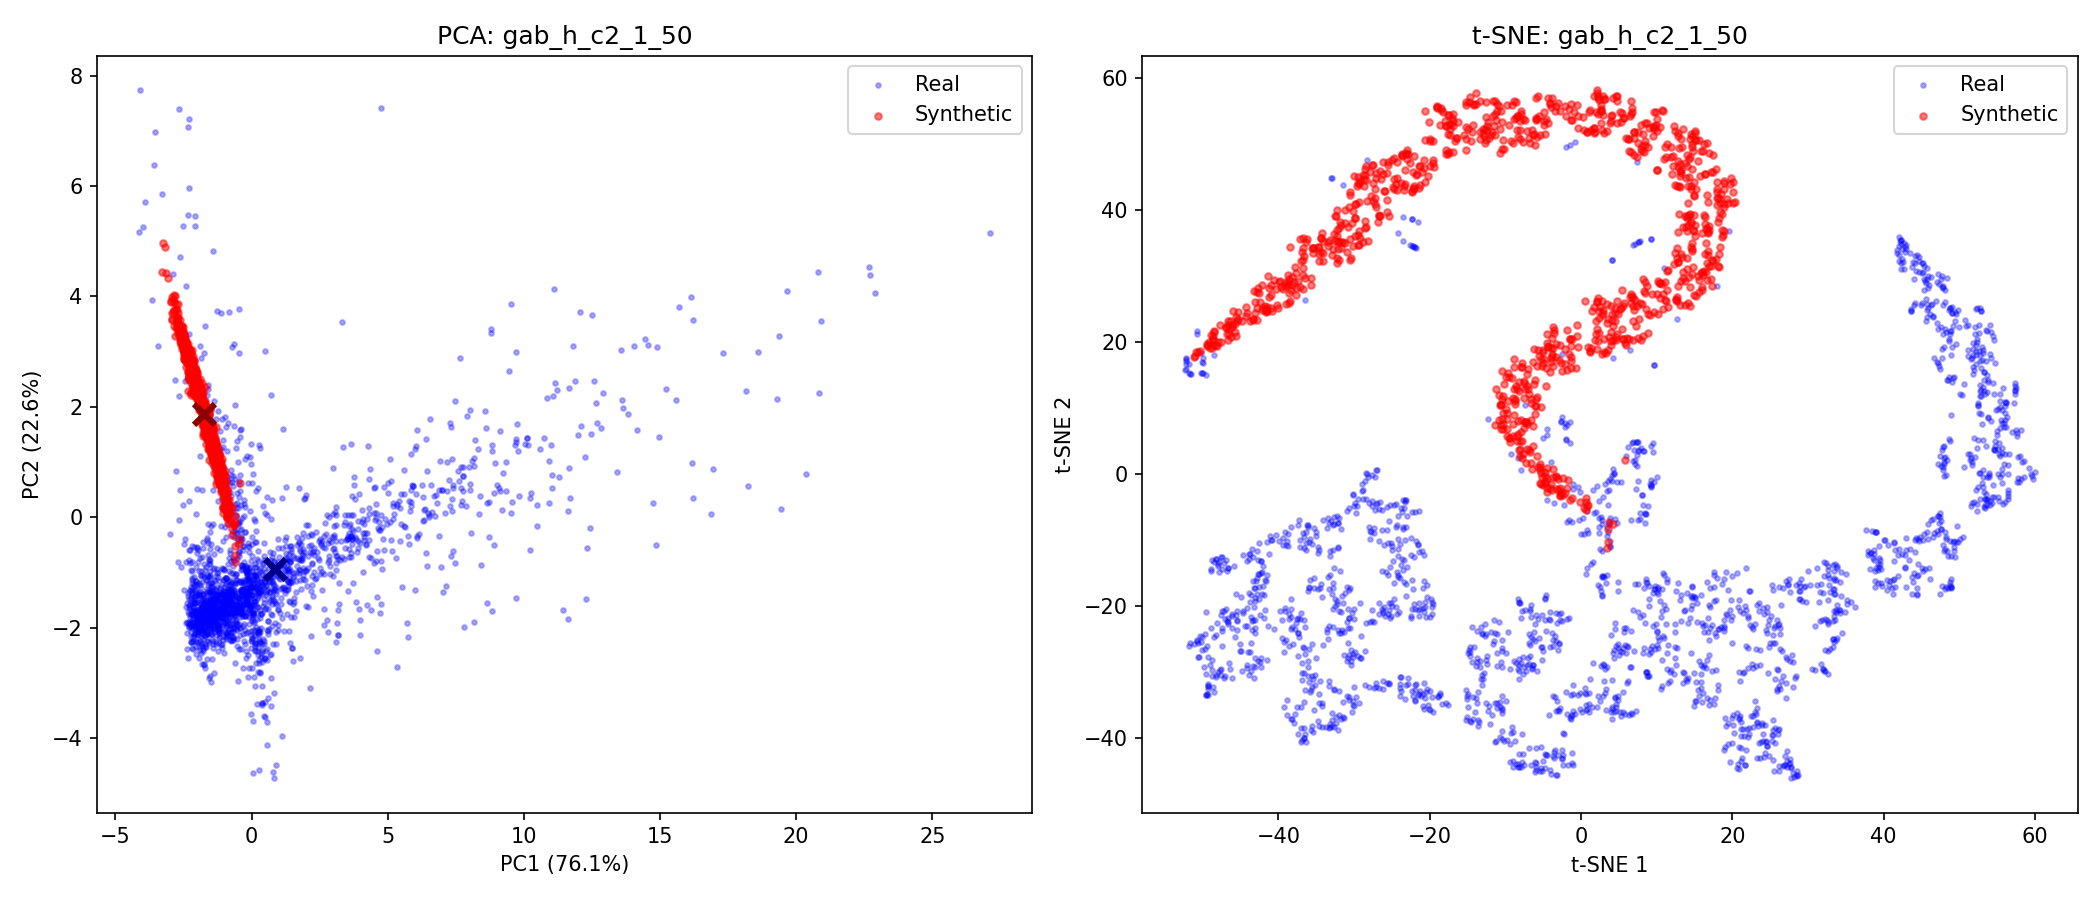
\includegraphics[width=\textwidth]{figures/gab_h_c2_1_50_gcn_visualization.png}
		\caption{Config 2, NM=1 (LR=0.0005)}
	\end{subfigure}
	\hfill
	\begin{subfigure}[b]{0.48\textwidth}
		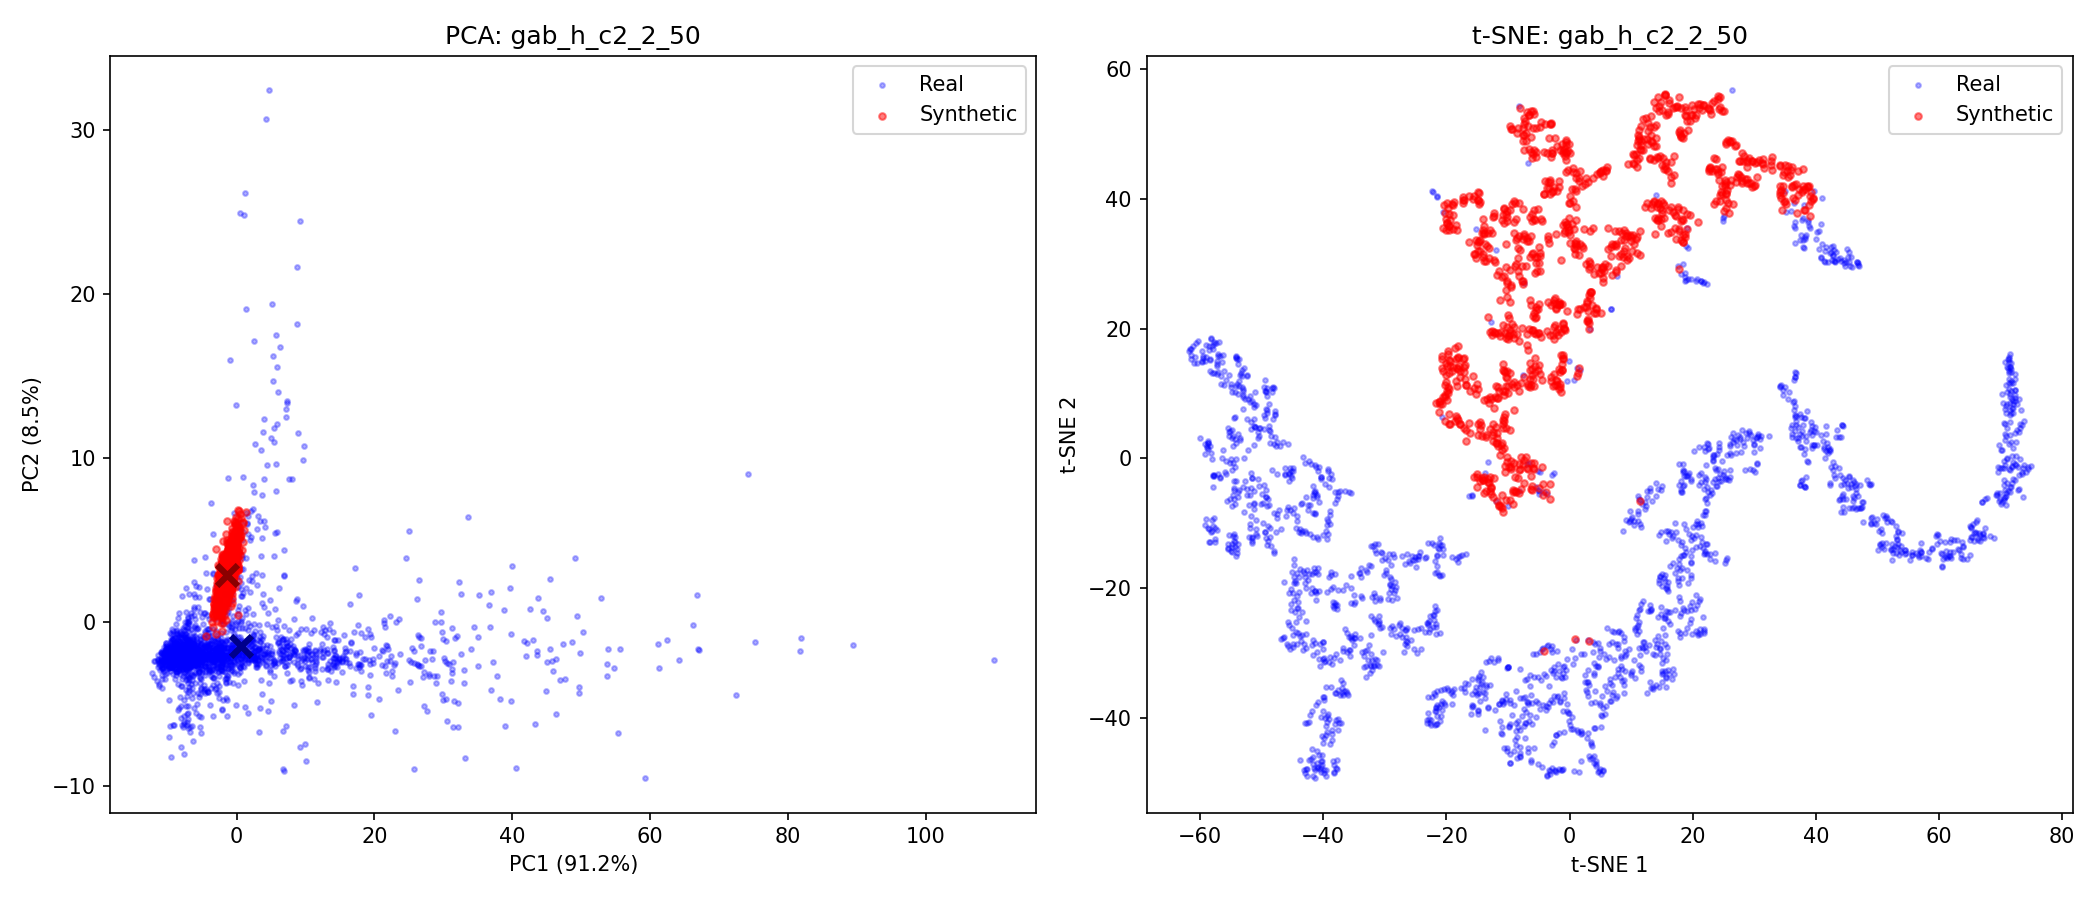
\includegraphics[width=\textwidth]{figures/gab_h_c2_2_50_gcn_visualization.png}
		\caption{Config 2, NM=2 (LR=0.0005)}
	\end{subfigure}
	\caption{PCA and t-SNE visualization of GCN embeddings for Incremental implementation. Blue points represent real users, red points represent synthetic users.}
	\label{fig:gcn_incremental}
\end{figure}

Table~\ref{tab:pca_stats} summarizes the PCA statistics for each configuration, including the explained variance ratio and the centroid distance between real and synthetic user embeddings.

\begin{table}[h]
	\centering
	\caption{PCA statistics for GCN embeddings}
	\label{tab:pca_stats}
	\small
	\begin{tabular}{llcccc}
		\toprule
		 & \textbf{Config} & \textbf{PC1}       & \textbf{PC2}       & \textbf{Total}     & \textbf{Centroid} \\
		 &                 & \textbf{Explained} & \textbf{Explained} & \textbf{Explained} & \textbf{Distance} \\
		\midrule
		\multirow{4}{*}{\rotatebox{90}{\textbf{Orig.}}}
		 & Config 1, NM=1  & 99.98\%            & 0.01\%             & 100.00\%           & 6.29              \\
		 & Config 1, NM=2  & 99.71\%            & 0.23\%             & 99.94\%            & 2.33              \\
		 & Config 2, NM=1  & 95.99\%            & 3.39\%             & 99.38\%            & 2.06              \\
		 & Config 2, NM=2  & 99.96\%            & 0.03\%             & 100.00\%           & 6.65              \\
		\midrule
		\multirow{4}{*}{\rotatebox{90}{\textbf{Incr.}}}
		 & Config 1, NM=1  & 99.65\%            & 0.21\%             & 99.86\%            & 1.01              \\
		 & Config 1, NM=2  & 99.39\%            & 0.57\%             & 99.96\%            & 3.41              \\
		 & Config 2, NM=1  & 76.13\%            & 22.61\%            & 98.74\%            & 3.84              \\
		 & Config 2, NM=2  & 91.20\%            & 8.47\%             & 99.67\%            & 4.78              \\
		\bottomrule
	\end{tabular}
\end{table}

The analysis reveals several key observations:

\paragraph{Dimensional Collapse and Oversmoothing.} The Original implementation configurations show extreme concentration in the first principal component (95-100\%), indicating \textbf{dimensional collapse}: the GCN embeddings collapse to a nearly one-dimensional space. This phenomenon is closely related to \textbf{oversmoothing} in Graph Neural Networks, where repeated message passing operations cause node representations to become indistinguishable from one another \cite{liDeeperInsightGraph2018,oonoGraphNeuralNetworks2020}. After multiple GCN layers, each node's embedding becomes dominated by the aggregated neighborhood statistics rather than its individual features.

In contrast, the Incremental implementation shows more variance distribution: Config 2 with NM=1 achieves only 76.13\% on PC1, with 22.61\% on PC2, suggesting a richer embedding space with less severe oversmoothing. This may explain why that particular run is the only one that attempts to connect synthetic users, even if with poor performance.

\paragraph{Centroid Distance.} The centroid distance between real and synthetic embeddings correlates strongly with classification performance:
\begin{itemize}
	\item \textbf{Original Config 1 NM=1 (6.29)} and \textbf{Config 2 NM=2 (6.65)}: Excellent separation, aligning with the highest MAP scores (0.8660) and balanced F1.
	\item \textbf{Incremental Config 1 NM=1 (1.01)}: Poor separation, correlated to the fact that the model predicts exclusively Class 1.
	\item \textbf{Incremental Config 2 NM=1 (3.84)} and \textbf{Config 2 NM=2 (4.78)}: Moderate separation with richer embedding structure (lower PC1 explained variance).
\end{itemize}

We can say that the failure in connecting synthetic users for the original configurations is due to the fact that the model learns a very narrow embedding space where real and synthetic users are perfectly separated, but the synthetic users are clustered in a single point, so the model is not able to learn any discriminative feature for them, and it ends up predicting always 0 for the edges between synthetic users. On the other hand, the incremental approach that link synthetic users is the one with the lowest explained variance on PC1, and the highest explained variance on PC2, so the model learns a richer embedding space where real and synthetic users are not perfectly separated, but the synthetic users are spread across the space, so the model is able to learn some discriminative features for them, even if with poor performance.

\paragraph{Effect of Negative Sampling.} Increasing NM from 1 to 2 generally improves centroid distance separation, particularly for the Incremental approach (1.01 $\rightarrow$ 3.41 for Config 1). This confirms that higher negative sampling encourages the model to learn more discriminative features.

% \paragraph{Original vs. Incremental Trade-off.} The Original approach achieves better separation (higher centroid distances) but with collapsed embedding dimensions. The Incremental approach produces more distributed embeddings but struggles with class separation, particularly with low negative sampling. This suggests a trade-off between embedding richness and discriminative power.

% The t-SNE visualizations complement these findings: real users form dense central clusters in configurations with high explained variance on PC1, while synthetic users spread across the periphery.

% \subsection*{Link Prediction Task}

% \subsection*{Populating the synthetic graph}

% \subsection*{Network metrics}

% Table~\ref{tab:social_network_metrics} presents the graph structural metrics for the Gab dataset compared to established social network datasets (Facebook, Twitter, Google+). The metrics include the number of nodes and edges, average degree, average path length, modularity, and clustering coefficient.

% \begin{table}[H]
% 	\centering
% 	\caption{Structural metrics comparison}
% 	\label{tab:social_network_metrics}
% 	\begin{tabular}{
% 			l
% 			S[table-format=5.0]
% 			S[table-format=8.0]
% 			S[table-format=2.2]
% 			S[table-format=1.2]
% 			S[table-format=1.2]
% 			S[table-format=1.2]
% 		}
% 		\toprule
% 		\textbf{Network}        &
% 		\textbf{Nodes}          &
% 		\textbf{Edges}          &
% 		\textbf{Avg Deg}        &
% 		\textbf{Avg Path}       &
% 		\textbf{Mod}            &
% 		\textbf{Clust. Coef.}                                                     \\
% 		\midrule
% 		Facebook                & 4039   & 88234    & 43.69  & 3.69 & 0.83 & 0.61 \\
% 		Twitter                 & 81306  & 1768149  & 21.75  & 4.91 & 0.80 & 0.57 \\
% 		Google+\footnotemark[4] & 107614 & 13673453 & 127.06 & 3.32 & 0.47 & 0.49 \\
% 		Gab (Ours)              & 25569  & 820910   & 32.11  & 3.08 & 0.24 & 0.08 \\
% 		\bottomrule
% 	\end{tabular}
% \end{table}
% \footnotetext[1]{https://snap.stanford.edu/data/ego-Facebook.html}
% \footnotetext[2]{https://snap.stanford.edu/data/ego-Twitter.html}
% \footnotetext[3]{https://snap.stanford.edu/data/ego-Gplus.html}
% \footnotetext[4]{Due to the dimension of the Google+ dataset, we report the metrics for the largest connected component (LCC) considering the 20\% of nodes with the highest degree.}

% The Gab dataset exhibits notably lower clustering coefficient (0.08) compared to other social networks (0.49-0.61), suggesting weaker local community structure and less triadic closure. The modularity of 0.24 is also lower than Facebook (0.83) and Twitter (0.80), indicating weaker community boundaries. However, the average path length of 3.08 is comparable to Facebook (3.69) and Google+ (3.32), confirming the ``small-world'' property typical of social networks.

% The lower clustering and modularity may reflect:
% \begin{itemize}
% 	\item The platform's specific user demographics and community structure
% 	\item Different interaction patterns compared to mainstream social networks
% 	\item The minimal content moderation creating different connection dynamics
% \end{itemize}

% Results from the experiments will be reported in this section once the training is completed. The evaluation will compare:
% \begin{itemize}
% 	\item The cumulative (standard) approach vs. the incremental approach
% 	\item Different feature configurations (degree-based vs. embedding-based)
% 	\item Both EvolveGCN-H and EvolveGCN-O variants where feasible
% \end{itemize}

% The structural properties of generated synthetic networks will be compared against the original Gab dataset and the baseline social networks shown in Table~\ref{tab:baseline_metrics}.


% \section{Evaluate Results}

% The evaluation assesses the extent to which the project meets the business success criteria defined in Chapter~\ref{cha:businessunderstanding}.

% \subsection*{Business Success Criteria Assessment}

% The business success criteria from Section~\ref{sec:business_success} are evaluated as follows:

% \begin{itemize}
% 	\item \textbf{Development of a temporal link prediction model based on EvolveGCN}: The model architecture has been implemented following the EvolveGCN-H variant, with support for both standard and incremental training pipelines.

% 	\item \textbf{Quantitative comparison using standard metrics}: The evaluation framework computes AUC-ROC, MAP, Precision, Recall, and F1-score as specified. Results are reported in Table~\ref{tab:results_comparison}, with the best configuration achieving MAP of 0.8660 (Original) and AUC of 0.8037 (Incremental).

% 	\item \textbf{Transfer learning for synthetic network generation}: The model can generate edge predictions on synthetic datasets, with structural analysis comparing degree distribution, clustering coefficient, average path length, and modularity against real networks. \textit{Status: Implementation complete, evaluation pending.}

% 	\item \textbf{Analysis of network evolution patterns}: The incremental training pipeline captures temporal dynamics through phase-by-phase adaptation. \textit{Status: Achieved.}

% 	\item \textbf{Generation of 1000-user synthetic network}: This objective requires completing experiments on the synthetic datasets. \textit{Status: Pending.}
% \end{itemize}

% \subsection*{Data Mining Success Criteria Assessment}

% The data mining success criteria from Section~\ref{sec:datamining_success} are evaluated:

% \begin{itemize}
% 	\item \textbf{High performance on link prediction tasks}: The best Original configuration achieves MAP of 0.8660 and Macro F1 of 0.8631, while the best Incremental configuration achieves AUC of 0.8037. Both approaches demonstrate effective temporal link prediction, with the Original approach showing superior classification performance and the Incremental approach showing better ranking quality (AUC).

% 	\item \textbf{Generalization to synthetic datasets}: The structural metrics comparison framework is in place. Generated networks will be evaluated for realism against Facebook, Twitter, Google+, and the original Gab network baselines.

% 	\item \textbf{Comprehensive insights on structural properties}: The GraphMetricsCalculator module computes all required metrics (average degree, clustering coefficient, modularity, shortest path length, community count).
% \end{itemize}



% \section{Review Process}

% The evaluation process follows an iterative approach:

% \begin{enumerate}
% 	\item \textbf{Phase-by-phase Review}: Each incremental training phase is reviewed immediately after completion, allowing for hyperparameter adjustments before the next phase.

% 	\item \textbf{Cross-validation}: For the standard approach, k-fold cross-validation ensures robustness of reported metrics.

% 	\item \textbf{Baseline Comparison}: Performance is compared against simple baselines:
% 	      \begin{itemize}
% 		      \item Random edge prediction
% 		      \item Preferential attachment (popular nodes get more connections)
% 		      \item Common neighbors heuristic (triadic closure)
% 	      \end{itemize}

% 	\item \textbf{Statistical Significance}: Bootstrap confidence intervals are computed for all metrics to assess reliability.
% \end{enumerate}



% \section{Determine Next Steps}

% Based on the current project status, the following next steps are recommended:

% \begin{enumerate}
% 	\item Complete training experiments on all six temporal snapshots
% 	\item Generate and evaluate synthetic networks using the trained models
% 	\item Compare incremental vs. standard approaches across all evaluation dimensions
% 	\item Document final results and prepare for potential deployment considerations
% \end{enumerate}
\titleformat{\chapter}[hang]{\Huge\bfseries}{\selectfont \thechapter\hsp\textcolor{red}{\emoji{rocket}}\hsp}{0pt}{\Huge\bfseries}

\chapter{Conclusion}

\pagestyle{fancy}

\bibliographystyle{unsrt} % plain, unsrt, alpha, abbrv
\bibliography{main}

\end{document}
